\pdfoutput=1

%%
%% This is file `sample-tinyml.tex',
%% generated with the docstrip utility.
%%
%% The original source files were:
%%
%% samples.dtx  (with options: `tinyml')
%%
%% IMPORTANT NOTICE:
%%
%% For the copyright see the source file.
%%
%% Any modified versions of this file must be renamed
%% with new filenames distinct from sample-tinyml.tex.
%%
%% For distribution of the original source see the terms
%% for copying and modification in the file samples.dtx.
%%
%% This generated file may be distributed as long as the
%% original source files, as listed above, are part of the
%% same distribution. (The sources need not necessarily be
%% in the same archive or directory.)
%%
%% The first command in your LaTeX source must be the \documentclass command.
\documentclass[tinyml]{acmart}

%%
%% \BibTeX command to typeset BibTeX logo in the docs
\AtBeginDocument{%
  \providecommand\BibTeX{{%
    \normalfont B\kern-0.5em{\scshape i\kern-0.25em b}\kern-0.8em\TeX}}}

%% Rights management information.  This information is sent to you
%% when you complete the rights form.  These commands have SAMPLE
%% values in them; it is your responsibility as an author to replace
%% the commands and values with those provided to you when you
%% complete the rights form.
\setcopyright{rightsretained}
%\setcopyright{none}
\copyrightyear{2025}
\acmYear{2025}

%% These commands are for a PROCEEDINGS abstract or paper.
% \acmConference[Woodstock '18]{Woodstock '18: ACM Symposium on Neural
%   Gaze Detection}{June 03--05, 2018}{Woodstock, NY}

%%
%% end of the preamble, start of the body of the document source.

\settopmatter{printacmref=false}

\usepackage{threeparttable}
\usepackage{pgfplots}
\pgfplotsset{compat=1.18}
\usepackage{tikz}
\usepackage{amsmath}
\usepackage{cases}
\usepackage{subfig}
\usepackage{xcolor,colortbl}
\usepackage{multirow}
\usepackage{url}
\usepackage{IEEEtrantools}

\usetikzlibrary{arrows.meta,positioning,automata}
\usetikzlibrary{backgrounds,positioning,shapes.gates.logic.US}
\usetikzlibrary{shapes.geometric}

% heatmap
\usepackage{collcell}
\usepackage{enumitem}

\setlength{\textfloatsep}{5pt}
\setlength{\intextsep}{5pt}

\begin{document}

%%
%% The "title" command has an optional parameter,
%% allowing the author to define a "short title" to be used in page headers.
\title{\textit{ETHEREAL}: Energy-efficient and High-throughput Inference using Compressed Tsetlin Machine}

%%
%% The "author" command and its associated commands are used to define
%% the authors and their affiliations.
%% Of note is the shared affiliation of the first two authors, and the
%% "authornote" and "authornotemark" commands
%% used to denote shared contribution to the research.
\iffalse
\author{Ben Trovato}
\authornote{Both authors contributed equally to this research.}
\email{trovato@corporation.com}
\orcid{1234-5678-9012}
\author{G.K.M. Tobin}
\authornotemark[1]
\email{webmaster@marysville-ohio.com}
\affiliation{%
  \institution{Institute for Clarity in Documentation}
  \streetaddress{P.O. Box 1212}
  \city{Dublin}
  \state{Ohio}
  \country{USA}
  \postcode{43017-6221}
}
\fi

\author{Shengyu Duan}
\affiliation{%
  \institution{Newcastle University}
  \city{Newcastle upon Tyne}
  \country{UK}}
\email{shengyu.duan@newcastle.ac.uk}

\author{Rishad Shafik}
\affiliation{%
  \institution{Newcastle University}
  \city{Newcastle upon Tyne}
  \country{UK}}
\email{rishad.shafik@newcastle.ac.uk}

\author{Alex Yakovlev}
\affiliation{%
  \institution{Newcastle University}
  \city{Newcastle upon Tyne}
  \country{UK}}
\email{alex.yakovlev@newcastle.ac.uk}

%%
%% By default, the full list of authors will be used in the page
%% headers. Often, this list is too long, and will overlap
%% other information printed in the page headers. This command allows
%% the author to define a more concise list
%% of authors' names for this purpose.
%\renewcommand{\shortauthors}{Trovato and Tobin, et al.}

%%
%% The abstract is a short summary of the work to be presented in the
%% article.
\begin{abstract}
The Tsetlin Machine (TM) is a novel alternative to deep neural networks (DNNs). Unlike DNNs, which rely on multi-path arithmetic operations, a TM learns propositional logic patterns from data literals using Tsetlin automata. This fundamental shift from arithmetic to logic underpinning makes TM suitable for empowering new applications with low-cost implementations. 

In TM, literals are often included by both positive and negative clauses within the same class, canceling out their impact on individual class definitions. This property can be exploited to develop compressed TM models, enabling energy-efficient and high-throughput inferences for machine learning (ML) applications.

We introduce a training approach that incorporates excluded automata states to sparsify TM logic patterns in both positive and negative clauses. This exclusion is iterative, ensuring that highly class-correlated (and therefore significant) literals are retained in the compressed inference model, ETHEREAL, to maintain strong classification accuracy. Compared to standard TMs, ETHEREAL TM models can reduce model size by up to 87.54\%, with only a minor accuracy compromise. We validate the impact of this compression on eight real-world Tiny machine learning (TinyML) datasets against standard TM, equivalent Random Forest (RF) and Binarized Neural Network (BNN) on the STM32F746G-DISCO platform. Our results show that ETHEREAL TM models achieve over an order of magnitude reduction in inference time (resulting in higher throughput) and energy consumption compared to BNNs, while maintaining a significantly smaller memory footprint compared to RFs.
\end{abstract}

%%
%% Keywords. The author(s) should pick words that accurately describe
%% the work being presented. Separate the keywords with commas.
\keywords{Tsetlin Machine, Machine Learning, Model Compression, TinyML}


%%
%% This command processes the author and affiliation and title
%% information and builds the first part of the formatted document.
\maketitle

\section{Introduction} \label{sec:intro}
The ever increasing demand for deploying machine learning (ML) in low-energy, resource-constrained edge applications presents a significant challenge for deep neural network (DNN) implementations due to their high computational demands. This has led to efforts to identify alternative low-complexity ML algorithms. One such alternative is the Tsetlin Machine (TM), which is a novel ML algorithm that has been demonstrated with lower complexity than DNN, while achieving comparable accuracy across a range of ML datasets and exhibiting inherent interpretability \cite{granmo2018tsetlin}. A TM marks a fundamental shift from DNN by relying primarily on logic operations, which for example could outperform a multi-layer neural network (NN) in terms of accuracy \cite{tang2024adatm}, while eliminating hundreds of thousands of multiply-accumulate operations.

Figure \ref{fig:tm_structure} demonstrates a typical TM structure for supervised ML. The structure comprises three incremental processes:
\begin{itemize}
	\item [A.]\textit{Booleanization}: Before TM training and inference regimes, the input dataset is first expressed in the form of a set of literals, represented as Boolean data. These literals are derived through a data encoding process, known as Booleanization. A typical Booleanization process uses fixed or dynamic thresholds to generate Boolean literals as opposed to Binarized features from the raw data \cite{9923830}.
	\item [B.]\textit{Training}: Booleanized literals are given to a group of clauses, each learning a sub-pattern of some literals and performing AND operations to independently make a decision. Each clause learns these patterns through Tsetlin Automata (TAs), which decide whether a literal is included (above middle state) or excluded (below middle state), after a reinforcement learning process, see Section \ref{sec:learn} for further details. Half of all clauses have positive/negative polarity, capturing sub-patterns to support/oppose a classification. 
	\item [C.]\textit{Inference}: A binary classification is performed by a majority vote between the sum of outputs from positive and negative clauses. A multi-class classification requires as many pairs of positive-negative clauses as classes, where the overall classification is based on the one with the greatest class sum.
\end{itemize}

\definecolor{new_red}{rgb}{0.95,0.47,0.47}
\definecolor{new_green}{rgb}{0.85,0.98,0.77}

\definecolor{dark_red}{rgb}{0.78,0.28,0.34}
\definecolor{dark_green}{rgb}{0.09,0.30,0.28}

\tikzset{
	node distance = 0pt,
	BB/.style args={#1/#2/#3}{% Building Box, options
		draw, semithick, 
		font=\small\linespread{0.84}\selectfont, align=center, 
		minimum width=#1, minimum height=#2, text depth=0.25ex, 
		fill=#3, outer sep=0pt}
} % end of tikzset

\tikzset{
	sectors/.style n args={6}{minimum width=#1, minimum height=#2, 
		text depth=0.25ex, outer sep=0pt,
		append after command={\pgfextra{\let\LN\tikzlastnode
				\draw[fill=#3]  (\LN.west)  -| (\LN.north)
				{[rounded corners=3mm] -- (\LN.north west)}
				{[rounded corners=3mm] -- cycle}
				;
				
    			\draw[fill=#5]  (\LN.east)  -| (\LN.north)
				{[rounded corners=3mm] -- (\LN.north east)}
				[rounded corners=3mm] -- cycle;
				;
	} } }
}

\begin{figure}[!htb]
\vspace{-0.2cm}
\centering
\begin{tikzpicture}
[        GateCfg/.style={
	logic gate inputs={normal,normal},
	draw,
	thick,
	scale=1
	},
	cross/.style={path picture={ 
			\draw[black]
			(path picture bounding box.south east) -- (path picture bounding box.north west) (path picture bounding box.south west) -- (path picture bounding box.north east);
	}},
	scale=0.5, every node/.style={scale=0.5}
]
% clause M
\begin{scope}[xshift=1.45cm,yshift=2.5cm]
\draw[draw=black,fill=white] (-1.2,-7) rectangle ++(10.3,9);
\draw[draw=black,fill=black!30!white] (-1.2,1.5) rectangle ++(10.3,0.5) node[pos=.5] {\large{\textbf{Clause M}}};

\node[rotate=45] at (3.5,1.15) {\large{\textbf{...}}};

\draw[thick,arrows={-Triangle[]}] (9.1,-1.7) -- (9.6,-1.7);
\node[trapezium, draw, thick, minimum width=1cm, trapezium left angle=45, trapezium right angle=135, trapezium stretches=true, minimum height=0.8cm, fill=white] at (9.83,-1.9) {};
\node[rotate=45] at (9.83,-1.9) {$C_{M}$};

\draw[thick,arrows={-Triangle[]}] (10.23,-1.7) -- (11.4,-1.7);
\node [draw,thick,circle,cross,minimum width=0.4 cm,fill=white]() at (11.6,-1.7){};
\draw[arrows={-Triangle[]}] (11.6,-2.3) -- (11.6,-1.9);
\node[fill=blue!50!white] at (11.6,-2.4) {-1};

\draw[thick] (11.8,-1.7) -- (12.8,-1.7);
\draw[thick,arrows={-Triangle[]}] (12.8,-1.7) -- (12.1,-3.65);
\end{scope}

% clause M-1
\begin{scope}[xshift=1.15cm,yshift=1.8cm]
\draw[draw=black,fill=white] (-1.2,-7) rectangle ++(10.3,9);
\draw[draw=black,fill=black!30!white] (-1.2,1.5) rectangle ++(10.3,0.5) node[pos=.5] {\large{\textbf{Clause M-1}}};

\node[rotate=45] at (3.5,1.15) {\large{\textbf{...}}};

\draw[thick,arrows={-Triangle[]}] (9.1,-2) -- (9.5,-2);
\node[trapezium, draw, thick, minimum width=1cm, trapezium left angle=45, trapezium right angle=135, trapezium stretches=true, minimum height=0.8cm, fill=white] at (9.8,-2) {};
\node[rotate=45] at (9.8,-2) {\footnotesize{$C_{M-1}$}};
\node[rotate=70] at (9.5,-2.8) {\large{\textbf{...}}};

\draw[thick,arrows={-Triangle[]}] (10.1,-2) -- (11.1,-2);
\node [draw,thick,circle,cross,minimum width=0.4 cm,fill=white]() at (11.3,-2){};
\draw[arrows={-Triangle[]}] (11.3,-2.6) -- (11.3,-2.2);
\node[fill=yellow!50!white] at (11.3,-2.7) {+1};

\draw[thick] (11.5,-2) -- (11.8,-2);
\draw[thick,arrows={-Triangle[]}] (11.8,-2) -- (12,-3);
\end{scope}

% clause 2
\begin{scope}[xshift=0.3cm,yshift=0.7cm]
\draw[draw=black,fill=white] (-1.2,-7) rectangle ++(10.3,9);
\draw[draw=black,fill=black!30!white] (-1.2,1.5) rectangle ++(10.3,0.5) node[pos=.5] {\large{\textbf{Clause 2}}};

\draw[thick,arrows={-Triangle[]}] (9.1,-2.2) -- (9.9,-2.2);
\node[trapezium, draw, thick, minimum width=1cm, trapezium left angle=45, trapezium right angle=135, trapezium stretches=true, minimum height=0.8cm, fill=white] at (10.13,-2.4) {};
\node[rotate=45] at (10.13,-2.4) {$C_2$};

\draw[thick,arrows={-Triangle[]}] (10.55,-2.2) -- (11.4,-2.2);
\node [draw,thick,circle,cross,minimum width=0.4 cm,fill=white]() at (11.6,-2.2){};
\draw[arrows={-Triangle[]}] (11.6,-2.8) -- (11.6,-2.4);
\node[fill=blue!50!white] at (11.6,-2.9) {-1};

\draw[thick,fill=white] (13.1,-2.2) circle [radius=0.4] node () {\large{$\sum$}};
\draw[thick,arrows={-Triangle[]}] (11.8,-2.2) -- (12.7,-2.2);

% class sum
\node[trapezium, draw, thick, minimum width=1cm, trapezium left angle=45, trapezium right angle=135, trapezium stretches=true, minimum height=0.8cm, fill=white] at (14.3,-2.4) {};
\draw[thick,arrows={-Triangle[]}] (13.5,-2.2) -- (14.05,-2.2);
\node[] at (14.6,-1.7) {\large{\textbf{Class Sum}}};

\end{scope}

% TA states 1
\begin{scope}[xshift=0cm,yshift=0cm]
\draw[draw=black,fill=white] (-1.2,-7) rectangle ++(10.3,9);
\draw[draw=black,fill=black!30!white] (-1.2,1.5) rectangle ++(10.3,0.5) node[pos=.5] {\large{\textbf{Clause 1}}};
\node[] at (2.75,1.05) {\large{\textbf{Tsetlin Automata Team}}};

\node at (2.75,-0.7) [sectors= {72mm}{28mm}
{new_red}{}
{new_green}{}] {};

\draw[thick,fill=white] (0,0) circle [radius=0.3] node (s1) {1};
\draw[thick, arrows={-Stealth[reversed,reversed]},dashed] (-0.3,-0.2) to [out=230,in=160,looseness=4] (-0.3,0.2);
\draw[thick,fill=white] (1,0) circle [radius=0.3] node (s2) {2};
\draw[thick, arrows={-Stealth[reversed,reversed]}] (0,0.3) to [bend left=45] (1,0.3);
\draw[thick, arrows={Stealth[reversed,reversed]-},dashed] (0,-0.3) to [bend right=45] (1,-0.3);
\draw[thick,fill=white] (2.2,0) circle [radius=0.3] node (sn) {N};
\node[] at (1.6,0) {...};
\draw[thick, arrows={-Stealth[reversed,reversed]}] (1,0.3) to [bend left=35] (2.2,0.3);
\draw[thick, arrows={Stealth[reversed,reversed]-},dashed] (1,-0.3) to [bend right=35] (2.2,-0.3);

\draw[thick, arrows={-Stealth[reversed,reversed]}] (2.2,0.3) to [bend left=35] (3.3,0.3);
\draw[thick, arrows={Stealth[reversed,reversed]-},dashed] (2.2,-0.3) to [bend right=35] (3.3,-0.3);

\draw[thick,fill=white] (3.3,0) circle [radius=0.3] node (sn1) {\footnotesize{N+1}};
\draw[thick, arrows={-Stealth[reversed,reversed]}] (3.3,0.3) to [bend left=45] (4.3,0.3);
\draw[thick, arrows={Stealth[reversed,reversed]-},dashed] (3.3,-0.3) to [bend right=45] (4.3,-0.3);
\draw[thick,fill=white] (4.3,0) circle [radius=0.3] node (sn2) {};
\draw[draw=none,fill=black!25!white] (4.3,0) circle [radius=0.24] node () {\footnotesize{N+2}};
\node[] at (4.9,0) {...};
\draw[thick, arrows={-Stealth[reversed,reversed]}] (4.3,0.3) to [bend left=35] (5.5,0.3);
\draw[thick, arrows={Stealth[reversed,reversed]-},dashed] (4.3,-0.3) to [bend right=35] (5.5,-0.3);
\draw[thick,fill=white] (5.5,0) circle [radius=0.3] node (s2n) {2N};
\draw[thick, arrows={-Stealth[reversed,reversed]}] (5.8,0.2) to [out=30,in=330,looseness=4] (5.8,-0.2);

\draw[ultra thick, arrows={-Triangle[]}] (6.5,0) to (7.1,0);
\node[] at (7.4,0) {\large{$x_0$}};

\draw[ultra thick, arrows={-Triangle[]}] (-1.6,0) to (-1,0);
\node[] at (-2.2,0) {\large{$x_0$}};
\end{scope}

% TA states 2
\begin{scope}[xshift=0cm,yshift=-1.6cm]
\node at (2.75,-0.7) [sectors= {72mm}{28mm}
{new_red}{}
{new_green}{}] {};

\draw[thick,fill=white] (0,0) circle [radius=0.3] node (s1) {1};
\draw[thick, arrows={-Stealth[reversed,reversed]},dashed] (-0.3,-0.2) to [out=230,in=160,looseness=4] (-0.3,0.2);
\draw[thick,fill=white] (1,0) circle [radius=0.3] node (s2) {2};
\draw[draw=none,fill=black!25!white] (1,0) circle [radius=0.24] node () {2};
\draw[thick, arrows={-Stealth[reversed,reversed]}] (0,0.3) to [bend left=45] (1,0.3);
\draw[thick, arrows={Stealth[reversed,reversed]-},dashed] (0,-0.3) to [bend right=45] (1,-0.3);
\draw[thick,fill=white] (2.2,0) circle [radius=0.3] node (sn) {N};
\node[] at (1.6,0) {...};
\draw[thick, arrows={-Stealth[reversed,reversed]}] (1,0.3) to [bend left=35] (2.2,0.3);
\draw[thick, arrows={Stealth[reversed,reversed]-},dashed] (1,-0.3) to [bend right=35] (2.2,-0.3);

\draw[thick, arrows={-Stealth[reversed,reversed]}] (2.2,0.3) to [bend left=35] (3.3,0.3);
\draw[thick, arrows={Stealth[reversed,reversed]-},dashed] (2.2,-0.3) to [bend right=35] (3.3,-0.3);

\draw[thick,fill=white] (3.3,0) circle [radius=0.3] node (sn1) {\footnotesize{N+1}};
\draw[thick, arrows={-Stealth[reversed,reversed]}] (3.3,0.3) to [bend left=45] (4.3,0.3);
\draw[thick, arrows={Stealth[reversed,reversed]-},dashed] (3.3,-0.3) to [bend right=45] (4.3,-0.3);
\draw[thick,fill=white] (4.3,0) circle [radius=0.3] node (sn2) {\footnotesize{N+2}};
\node[] at (4.9,0) {...};
\draw[thick, arrows={-Stealth[reversed,reversed]}] (4.3,0.3) to [bend left=35] (5.5,0.3);
\draw[thick, arrows={Stealth[reversed,reversed]-},dashed] (4.3,-0.3) to [bend right=35] (5.5,-0.3);
\draw[thick,fill=white] (5.5,0) circle [radius=0.3] node (s2n) {2N};
\draw[thick, arrows={-Stealth[reversed,reversed]}] (5.8,0.2) to [out=30,in=330,looseness=4] (5.8,-0.2);

\draw[ultra thick, arrows={-Triangle[]}] (-1.6,0) to (-1,0);
\node[] at (-2.2,0) {\large{$\overline{x_0}$}};
\end{scope}

% TA states 3
\begin{scope}[xshift=0cm,yshift=-3.2cm]
\node at (2.75,-0.7) [sectors= {72mm}{28mm}
{new_red}{}
{new_green}{}] {};

\draw[thick,fill=white] (0,0) circle [radius=0.3] node (s1) {1};
\draw[thick, arrows={-Stealth[reversed,reversed]},dashed] (-0.3,-0.2) to [out=230,in=160,looseness=4] (-0.3,0.2);
\draw[thick, arrows={-Stealth[reversed,reversed]}] (0,0.3) to [bend left=45] (1,0.3);
\draw[thick,fill=white] (1,0) circle [radius=0.3] node (s2) {2};
\draw[thick, arrows={Stealth[reversed,reversed]-},dashed] (0,-0.3) to [bend right=45] (1,-0.3);
\draw[thick,fill=white] (2.2,0) circle [radius=0.3] node (sn) {};
\draw[draw=none,fill=black!25!white] (2.2,0) circle [radius=0.24] node () {N};
\node[] at (1.6,0) {...};
\draw[thick, arrows={-Stealth[reversed,reversed]}] (1,0.3) to [bend left=35] (2.2,0.3);
\draw[thick, arrows={Stealth[reversed,reversed]-},dashed] (1,-0.3) to [bend right=35] (2.2,-0.3);

\draw[thick, arrows={-Stealth[reversed,reversed]}] (2.2,0.3) to [bend left=35] (3.3,0.3);
\draw[thick, arrows={Stealth[reversed,reversed]-},dashed] (2.2,-0.3) to [bend right=35] (3.3,-0.3);

\draw[thick,fill=white] (3.3,0) circle [radius=0.3] node (sn1) {\footnotesize{N+1}};
\draw[thick, arrows={-Stealth[reversed,reversed]}] (3.3,0.3) to [bend left=45] (4.3,0.3);
\draw[thick, arrows={Stealth[reversed,reversed]-},dashed] (3.3,-0.3) to [bend right=45] (4.3,-0.3);
\draw[thick,fill=white] (4.3,0) circle [radius=0.3] node (sn2) {\footnotesize{N+2}};
\node[] at (4.9,0) {...};
\draw[thick, arrows={-Stealth[reversed,reversed]}] (4.3,0.3) to [bend left=35] (5.5,0.3);
\draw[thick, arrows={Stealth[reversed,reversed]-},dashed] (4.3,-0.3) to [bend right=35] (5.5,-0.3);
\draw[thick,fill=white] (5.5,0) circle [radius=0.3] node (s2n) {2N};
\draw[thick, arrows={-Stealth[reversed,reversed]}] (5.8,0.2) to [out=30,in=330,looseness=4] (5.8,-0.2);

\draw[ultra thick, arrows={-Triangle[]}] (-1.6,0) to (-1,0);
\node[] at (-2.2,0) {\large{$x_1$}};
\end{scope}

% TA states 4
\begin{scope}[xshift=0cm,yshift=-4.8cm]
\node at (2.75,-0.7) [sectors= {72mm}{28mm}
{new_red}{}
{new_green}{}] {};

\draw[thick,fill=white] (0,0) circle [radius=0.3] node (s1) {1};
\draw[thick, arrows={-Stealth[reversed,reversed]},dashed] (-0.3,-0.2) to [out=230,in=160,looseness=4] (-0.3,0.2);
\draw[thick,fill=white] (1,0) circle [radius=0.3] node (s2) {2};
\draw[thick, arrows={-Stealth[reversed,reversed]}] (0,0.3) to [bend left=45] (1,0.3);
\draw[thick, arrows={Stealth[reversed,reversed]-},dashed] (0,-0.3) to [bend right=45] (1,-0.3);
\draw[thick,fill=white] (2.2,0) circle [radius=0.3] node (sn) {N};
\node[] at (1.6,0) {...};
\draw[thick, arrows={-Stealth[reversed,reversed]}] (1,0.3) to [bend left=35] (2.2,0.3);
\draw[thick, arrows={Stealth[reversed,reversed]-},dashed] (1,-0.3) to [bend right=35] (2.2,-0.3);

\draw[thick, arrows={-Stealth[reversed,reversed]}] (2.2,0.3) to [bend left=35] (3.3,0.3);
\draw[thick, arrows={Stealth[reversed,reversed]-},dashed] (2.2,-0.3) to [bend right=35] (3.3,-0.3);

\draw[thick,fill=white] (3.3,0) circle [radius=0.3] node (sn1) {\footnotesize{N+1}};
\draw[thick, arrows={-Stealth[reversed,reversed]}] (3.3,0.3) to [bend left=45] (4.3,0.3);
\draw[thick, arrows={Stealth[reversed,reversed]-},dashed] (3.3,-0.3) to [bend right=45] (4.3,-0.3);
\draw[thick,fill=white] (4.3,0) circle [radius=0.3] node (sn2) {\footnotesize{N+2}};
\node[] at (4.9,0) {...};
\draw[thick, arrows={-Stealth[reversed,reversed]}] (4.3,0.3) to [bend left=35] (5.5,0.3);
\draw[thick, arrows={Stealth[reversed,reversed]-},dashed] (4.3,-0.3) to [bend right=35] (5.5,-0.3);
\draw[thick,fill=white] (5.5,0) circle [radius=0.3] node (s2n) {};
\draw[draw=none,fill=black!25!white] (5.5,0) circle [radius=0.24] node () {2N};
\draw[thick, arrows={-Stealth[reversed,reversed]}] (5.8,0.2) to [out=30,in=330,looseness=4] (5.8,-0.2);

\draw[ultra thick, arrows={-Triangle[]}] (6.5,0) to (7.1,0);
\node[] at (7.4,0) {\large{$\overline{x_1}$}};

\draw[ultra thick, arrows={-Triangle[]}] (-1.6,0) to (-1,0);
\node[] at (-2.2,0) {\large{$\overline{x_1}$}};

\node[] at (1.2,-1.05) {\textcolor{dark_red}{\large{\textbf{Exclude}}}};
\node[] at (4.5,-1.05) {\textcolor{dark_green}{\large{\textbf{Include}}}};

\begin{scope}[xshift=0.9cm,yshift=0cm]
\draw[thick,fill=white] (-0.8,-1.8) circle [radius=0.22] node () {};
\node[] at (-0.12,-1.8) {State};
\draw[thick,fill=white] (0.8,-1.8) circle [radius=0.22] node () {};
\draw[draw=none,fill=black!25!white] (0.8,-1.8) circle [radius=0.17] node () {};
\node[] at (1.95,-1.8) {Active state};
\draw[thick, arrows={-Stealth[reversed,reversed]}] (3.05,-1.8) to (3.55,-1.8);
\node[] at (4.3,-1.8) {Increment};
\draw[thick, arrows={-Stealth[reversed,reversed]},dashed] (5.3,-1.8) to (5.8,-1.8);
\node[] at (6.65,-1.8) {Decrement};
\end{scope}

\end{scope}

% clause output
\node[] at (-2.2,0.6) {\large{\textbf{Literal}}};
\draw[] (-2,0.2) -- ++(0.1,0) |- (-2,-5);
\draw[] (-2.45,0.2) -- ++(-0.1,0) |- (-2.45,-5);
\path (8.5,-2.5) node[and gate US,GateCfg] (AND1) {};
\draw[thick] (7.7,0) -- ++(0.1,0) |- (AND1.input 1); 
\draw[thick] (7.7,-4.8) -- ++(0.1,0) |- (AND1.input 2);
\node [draw,thick,circle,cross,minimum width=0.4 cm,fill=white]() at (11.3,-2.5){};
\draw[thick,arrows={-Triangle[]}] (AND1.output) -- (9.75,-2.5);

\node[trapezium, draw, thick, minimum width=1cm, trapezium left angle=45, trapezium right angle=135, trapezium stretches=true, minimum height=0.8cm, fill=white] at (10.1,-2.5) {};
\node[rotate=45] at (10.1,-2.5) {$C_1$};

\draw[thick,arrows={-Triangle[]}] (10.4,-2.5) -- (11.1,-2.5);
\draw[arrows={-Triangle[]}] (11.3,-3) -- (11.3,-2.7);
\node[fill=yellow!50!white] at (11.3,-3.2) {+1}; 

\node[] at (11.3,1.3) {\large{\textbf{Clause Output}}};

\draw[thick] (11.5,-2.5) -- (12.8,-2.5);
\draw[thick,arrows={-Triangle[]}] (12.8,-2.5) -- (13.2,-1.8);

\node[fill=yellow!50!white] at (11.3,-5) {+1};
\node[] at (12.9,-5) {Positive polarity};
\node[fill=blue!50!white] at (11.3,-5.6) {-1};
\node[] at (12.9,-5.6) {Negative polarity};
\end{tikzpicture}

\caption{The TM structure.}
\label{fig:tm_structure}
\Description[overall TM structure]

\vspace{-0.2cm}

\end{figure}


After training, TA array exhibits high sparsity; for example in the case of an MNIST dataset there are more than 99\% excludes. This property was leveraged to derive a compact model representation, REDRESS \cite{maheshwari2023redress}. The model only stores the information of includes as relative clauses and literal addressing. However, 
REDRESS, applied as a post-training compression, still follows the standard training process of the vanilla TM, resulting in a sparse form of training where the number of includes is not minimized, retaining less relevant or irrelevant context.
Reducing the number of includes is important in TMs, as their inherent sparse nature often incorporates literals with weak correlation to the target classes.  

It is possible to develop a more efficient TM by eliminating literals with weak correlations to a class, leading to minimal accuracy loss. 
{Though extensive research has been conducted on pruning weakly correlated features in DNNs, we emphasize that TM employs fundamentally different learning mechanism and data representation, and thus the pruning methods for DNNs are not applicable.}
In this work, we leverage the inherent interpretability of TM to identify weakly correlated literals, which are often included in both positive and negative clauses, due to their lack of strong association with a class. We propose a training approach to remove these literals, compressing TM models at the algorithm level, beyond REDRESS. This method, called \textbf{ETHEREAL}, enables \textbf{E}nergy-efficien\textbf{T}, \textbf{H}igh-throughput and accurate inf\textbf{E}rence through the practical implementation of a comp\textbf{RE}ssed tset\textbf{L}in m\textbf{A}chine. 

ETHEREAL introduces an additional exclusion process during training, to exclude literals shared by positive and negative clauses.
The exclusion is iteratively followed by standard training to restore important features. Results from eight real-world Tiny Machine Learning (TinyML) datasets show that ETHEREAL can realize up to an 87.54\% reduction in model size with a maximum accuracy loss of only 3.38\%, compared to a vanilla TM \cite{granmo2018tsetlin}. In some cases, accuracy even improves by eliminating some features that contribute noise. We use STM32F746G-DISCO micro-controller as the platform to implement ETHEREAL alongside REDRESS TM \cite{maheshwari2023redress}, a Random Forest (RF) and a Binarized Neural Network (BNN) \cite{courbariaux2016binarized, geiger2020larq}. The TM implementations can provide up to an order of magnitude reduction in inference time and energy compared to BNN, and 7$\times$ lower memory footprints than RF, while giving comparable accuracy. ETHEREAL further improves these design metrics, commensurate with the model size reductions achieved over REDRESS TMs. 

In this paper, we make the following key \textbf{\textit{contributions}}:
\begin{itemize}
	\item Empirical evidence revealing the inefficiency of vanilla TM in including less correlated (and thereby insignificant) literals.
	\item A training approach with additional exclusion, effectively compressing TM model and ensuring high accuracy.
	\item Validation with TinyML benchmarks on STM32 micro-controller, validating improved throughput, energy and memory usage produced by ETHEREAL. 
\end{itemize}

%We describe the TM learning process in Section \ref{sec:learn}. The ETHEREAL model compression method is introduced and evaluated in Sections \ref{sec:ethereal} and \ref{sec:eva}, respectively. We conclude our work in Section \ref{sec:conc}.

\section{TM Learning Dynamics} \label{sec:learn}
A TM is trained to capture the sub-pattern supporting or opposing a proposition by adjusting the TA states, which determine inclusion or exclusion of literals, driven by Type I and Type II feedback.

Figure \ref{fig:tm_feedbacks} explains the conditions under which each type of feedback is initiated. For a TA with 2N states, all TA states are initially set to either N or N+1 at random ($i.e.$, near the confusion state). During training, feedback is probabilistically activated for each datapoint; each specific type of feedback as well as the TAs being reinforced are determined by the training outcomes at the class and clause levels. 
%In Figure \ref{fig:tm_feedbacks}, $y$ indicates the label of a sample: for binary classification, $y$=1 or 0 suggests the sample belongs to the class or not, respectively; for multiclass classification and a TM for a certain class, $y$=1 or 0 suggests the sample belongs to the class or any other classes, respectively. 
%At a datapoint, each clause independently receives its feedback, the type of which is determined by both $y$ and the clause polarity: 
%\todo{This line repeats what you said earlier with a bit more specificity -- keep one; you actually repeat again in the following paragraph}
Type I/II feedback is activated for all positive/negative clauses when $y$=1, while an opposite reaction occurs when $y$=0.

\begin{figure}[!htb]
\centering

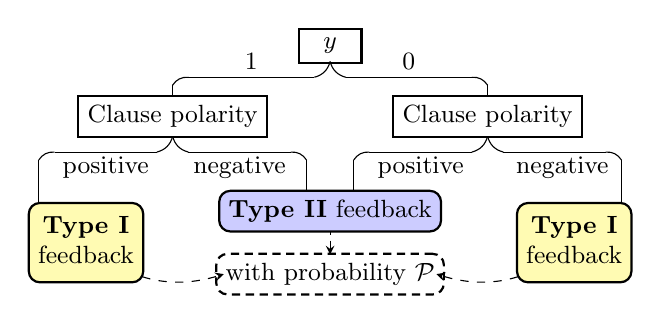
\begin{tikzpicture}[font=\small]
\node [draw, thick, shape=rectangle, minimum width=0.8cm] at (0,-0.3) {$y$};
\draw []  (0,-0.5) to [bend left] (-0.2,-0.7);
\draw [] (-0.2,-0.7) -- (-1.8,-0.7);
\node[] at (-1,-0.5) {1};
\draw []  (-1.8,-0.7) to [bend right] (-2,-0.8);
\draw [] (-2,-0.8) -- (-2,-1.25);
\draw []  (0,-0.5) to [bend right] (0.2,-0.7);
\draw [] (0.2,-0.7) -- (1.8,-0.7);
\node[] at (1,-0.5) {0};
\draw []  (1.8,-0.7) to [bend left] (2,-0.8);
\draw [] (2,-0.8) -- (2,-1.25);

\draw []  (-2,-1.45) to [bend left] (-2.2,-1.65);
\draw [] (-2.2,-1.65) -- (-3.5,-1.65);
\node[] at (-2.85,-1.85) {positive};
\draw[] (-3.5,-1.65) to [bend right] (-3.7,-1.75);
\draw[] (-3.7,-1.75) -- (-3.7,-3);
\draw []  (-2,-1.45) to [bend right] (-1.8,-1.65);
\draw [] (-1.8,-1.65) -- (-0.5,-1.65);
\node[] at (-1.15,-1.85) {negative};
\draw[] (-0.5,-1.65) to [bend left] (-0.3,-1.75);
\draw[] (-0.3,-1.75) -- (-0.3,-2.6);
\node [draw, thick, shape=rectangle, minimum width=0.8cm,fill=white] at (-2,-1.2) {Clause polarity};

\draw [-stealth,dashed]  (-3.1,-2.8) to [bend right] (-1.35,-3.2);

\node [draw, thick, shape=rectangle, minimum width=0.8cm, rounded corners, fill=yellow!30!white] at (-3.1,-2.8) {\begin{tabular}[c]{@{}c@{}} \textbf{Type I} \\ feedback \end{tabular}};

\draw []  (2,-1.45) to [bend left] (1.8,-1.65);
\draw [] (1.8,-1.65) -- (0.5,-1.65);
\node[] at (1.15,-1.85) {positive};
\draw[] (0.5,-1.65) to [bend right] (0.3,-1.75);
\draw[] (0.3,-1.75) -- (0.3,-2.6);
\draw []  (2,-1.45) to [bend right] (2.2,-1.65);
\draw [] (2.2,-1.65) -- (3.5,-1.65);
\node[] at (2.95,-1.85) {negative};
\draw[] (3.5,-1.65) to [bend left] (3.7,-1.75);
\draw[] (3.7,-1.75) -- (3.7,-2.6);
\node [draw, thick, shape=rectangle, minimum width=0.8cm,fill=white] at (2,-1.2) {Clause polarity};

\draw [-stealth, dashed]  (3.1,-2.8) to [bend left] (1.35,-3.2);

\node [draw, thick, shape=rectangle, minimum width=0.8cm, rounded corners, fill=yellow!30!white] at (3.1,-2.8) {\begin{tabular}[c]{@{}c@{}} \textbf{Type I}  \\ feedback \end{tabular}};

\draw [-stealth, densely dashed] (0,-2.6) -- (0,-2.95);

\node [draw, thick, shape=rectangle, minimum width=0.8cm, rounded corners, fill=blue!20!white] at (0,-2.4) {\textbf{Type II} feedback};

\node [draw, densely dashed, thick, shape=rectangle, minimum width=0.8cm, rounded corners] at (0,-3.2) {with probability $\mathcal{P}$};

\end{tikzpicture}

\caption{TM feedback procedure, independently performed for each clause. For binary classification, $y$=1 or 0 suggests the sample belongs to the class or not, respectively; for multiclass classification and a TM for a certain class, $y$=1 or 0 suggests the sample belongs to the class or other classes, respectively.}
\label{fig:tm_feedbacks}

\Description[overall TM feedback]

\end{figure}


Figure \ref{fig:tm_feedbacks} shows both types of feedback are triggered with probability $\mathcal{P}$, determined by a hyperparameter $T$, as in (\ref{eq:feedback_prob}):
\vspace{-0.2cm}
\begin{IEEEeqnarray}{rCl}
	\mathcal{P} =\dfrac{T+(-1)^y\times\textrm{clip}(\sum\limits_{j=1}^{M} p_j C_j, -T, T)}{2T}
	\label{eq:feedback_prob}
\end{IEEEeqnarray}
where $M$ is the number of clauses; $p_j$ and $C_j$ are the polarity and output, respectively, for a specific clause. According to (\ref{eq:feedback_prob}), the farther the class sum is from $T$/$-T$ when $y$=1/0, the more likely the feedback is triggered, potentially calibrating more clauses to cast correct votes. On the other hand, feedback is withheld if the class sum becomes greater/smaller than $T$/$-T$, when $y$=1/0. Therefore, $T$ reveals the confidence in distinguishing between different classes. 

Figure \ref{fig:type_i_ii} illustrates the mechanism of both types of feedback.
%In Type I feedback (Figure \ref{fig:type_i_ii} (a)), the TA state of a literal tends to increase, if the literal for the current training sample is `1' and the clause with positive/negative polarity manages to support for the fact that $y$=1/0 by producing the clause output as `1'. 
%Thus, in general, a clause that correctly produces the output is likely to include more literals equaling `1' at the datapoint, through Type I feedback. 
In Type I feedback (Figure \ref{fig:type_i_ii} (a)), a clause that correctly supports or opposes the class (by producing an output of `1') is likely to include more literals that equal `1' at the datapoint.
%\todo{avoid potentially -- use probabilistically or don't use at all.}
This enables it to continue making the right decision by using a more fine-grained sub-pattern. On the other hand, the TA state of a literal equal to `0' is decreased to prevent it from overturning the correct output. 

Finally, a clause that fails to support the correct class (by producing an output of `0') may cause a false negative.
As a result, all TA of the clause are penalized by decreasing their states. 
In other words, Type I feedback combats false negatives by denying established sub-patterns and regenerating them in later learning process.

\definecolor{new_red}{rgb}{0.95,0.47,0.47}
\definecolor{new_green}{rgb}{0.85,0.98,0.77}

\begin{figure}[!htb]
\vspace{-0.5cm}
\centering
\subfloat[]{
\begin{tikzpicture}[font=\small]
\node [draw=none, shape=rectangle, minimum width=0.8cm, rounded corners, fill=yellow!30!white] at (0,0.6) {\textbf{Type I} Feedback};

\draw []  (0,-0.25) to [bend left] (-0.2,-0.45);
\draw [] (-0.2,-0.45) -- (-1.1,-0.45);
\node[] at (-0.65,-0.6) {1};
\draw []  (-1.1,-0.45) to [bend right] (-1.3,-0.55);
\draw [->] (-1.3,-0.55) -- (-1.3,-0.95);

\draw []  (0,-0.25) to [bend right] (0.2,-0.45);
\draw [] (0.2,-0.45) -- (1.1,-0.45);
\node[] at (0.65,-0.6) {0};
\draw []  (1.1,-0.45) to [bend left] (1.3,-0.55);
\draw [->] (1.3,-0.55) -- (1.3,-2.15);
\node [draw, thick, shape=rectangle, minimum width=0.8cm, fill=white] at (0,0) {Clause output};

\node [draw, thick, shape=rectangle, minimum width=0.8cm] at (-1.3,-1.18) {Literal};
\draw[->] (-1.3,-1.4) -- (-1.3,-2.15);
\node[] at (-1.45,-1.775) {1};
\draw[] (-1.3,-1.4) to [bend right] (-1.1,-1.6);
\draw[] (-1.1,-1.6) -- (1.1,-1.6);
\draw[] (1.1,-1.6) to [bend left] (1.3,-1.7);
\node[] at (0,-1.775) {0};

\node [draw, thick, shape=rectangle, minimum width=0.8cm, rounded corners, fill=new_green] at (-1.35,-2.8) {\begin{tabular}[c]{@{}c@{}} TA state \\ \textbf{increments} with \\ probability $\frac{s-1}{s}$ \end{tabular}};

\node [draw, thick, shape=rectangle, minimum width=0.8cm, rounded corners, fill=new_red!50!white] at (1.35,-2.8) {\begin{tabular}[c]{@{}c@{}} TA state \\ \textbf{decrements} with \\ probability $\frac{1}{s}$ \end{tabular}};

\end{tikzpicture}
}
\hspace{0.2cm}
\subfloat[]{
\begin{tikzpicture}[font=\small]
\node [draw=none, shape=rectangle, minimum width=0.8cm, rounded corners, fill=blue!20!white] at (0,0.6) {\textbf{Type II} Feedback};

\draw [->]  (0,-1.4) -- (0,-2.15);
\node[] at (-0.15,-1.775) {0};
\node [draw, thick, shape=rectangle, minimum width=0.8cm, fill=white] at (0,0) {Clause output};
	
\draw [->]  (0,-0.25) -- (0,-0.95);
\node[] at (-0.15,-0.6) {1};
\node [draw, thick, shape=rectangle, minimum width=0.8cm,fill=white] at (0,-1.2) {Literal};

\node [draw, thick, shape=rectangle, minimum width=2cm, minimum height=1.32cm, rounded corners, fill=new_green] at (0,-2.8) {\begin{tabular}[c]{@{}c@{}} TA state \\ \textbf{increments} \end{tabular}};
	
\end{tikzpicture}
}
\vspace{-0.2cm}
\caption{(a) Type I and (b) Type II feedback, where TA state remains unchanged for any other cases.}
\label{fig:type_i_ii}

\Description[Type I/II feedback]

\end{figure}


The probability of changing a TA state is determined by another hyperparameter, $s$, which indicates the probability of including a literal. The larger the value of $s$, the more/less likely a literal is to be included/excluded through Type I feedback. So far, the optimal values for both $T$ and $s$ are determined based on extensive trials aimed at achieving optimal accuracy~\cite{maheshwari2023redress, tarasyuk2023systematic}. 

If a clause incorrectly supports a class proposition, a false positive may occur. For instance, a positive/negative clause output is `1', when $y$=0/1. False positives are minimized by Type II feedback (Figure \ref{fig:type_i_ii} (b)). This type of feedback increases the TA states for the literals equaling `0', which potentially modifies the incorrect clause output of `1'. The TA states of a clause with output as `0' keeps unchanged, to avoid being trapped by local minima.

\section{ETHEREAL Model Compression} \label{sec:ethereal} 
%This section presents evidence of inefficiency in vanilla TM due to the inclusion of insignificant literals based on a case study, followed by the ETHEREAL to address this issue.
\subsection{Literal Significance in Learning Dynamics}
The TM feedback mechanism given in Figure \ref{fig:type_i_ii}
ensures faster convergence during the training regime, through the interactions between both types of feedback. 
In addition, accuracy generally improves as more literals are included to capture fine-grained sub-patterns, as described in Section \ref{sec:learn}. However, this training process overlooks the significance or the correlation of individual literals to the target class. For example, a literal that consistently equals `1' does not provide useful information for classification, yet it can still be included in many clauses without adversely affecting accuracy.
%Nevertheless, as the training proceeds, a TM always keeps expanding by including more literals. This is because: 1) it is only possible to exclude a literal from a clause through Type I feedback, and 2) in Type I feedback, the probability of increasing a TA state will be greater than that of decreasing it, if $s$ is greater than 2, which is unfortunately the case for nearly all reported TM models with good accuracy.

We conduct an exploratory experiment to demonstrate how a TM model expands during training. In our experiment, the TM is trained to classify MNIST handwritten digits~\cite{deng2012mnist}, chosen as a case study for its simplicity in visualizing such an image classification task for our later analysis. We set the number of clauses per class, $T$ and $s$ to 100, 10 and 3, respectively, and Booleanize the dataset by applying a threshold of 75 to all grayscale values. Figure \ref{fig:TM_acc_size} shows resulting test accuracy and model size. As can be seen, the accuracy tends to increase with more training epochs, which is accompanied by a large increment on number of includes. This trend of model expansion is seen to hold across datasets and hyperparameters, as more TAs are included through random selection of automata reinforcements through $s$ and $T$ parameters explained above.

We compare the performance of agents trained on data from the InSTA pipeline to agents trained on human demonstrations from WebLINX \citep{WebLINX} and Mind2Web \citep{Mind2Web}, two recent and popular benchmarks for web navigation. Recent works that mix synthetic data with real data control the real data sampling probability in the batch $p_{\text{real}}$ independently from data size \citep{DAFusion}. We employ $p_{\text{real}} = 0.5$ in few-shot experiments and $p_{\text{real}} = 0.8$ otherwise. Shown in Figure~\ref{fig:data-statistics}, our data have a wide spread in performance, so we apply several filtering rules to select high-quality training data. First, we require the evaluator to return \texttt{conf} = 1 that the task was successfully completed, and that the agent was on the right track (this selects data where the actions are reliable, and directly caused the task to be solved). Second, we filter data where the trajectory contains at least three actions. Third, we remove data where the agent encountered any type of server error, was presented with a captcha, or was blocked at any point. These steps produce $7,463$ high-quality demonstrations in which agents successfully completed tasks on diverse websites. We sample 500 demonstrations uniformly at random from this pool to create a diverse test set, and employ the remaining $6,963$ demonstrations to train agents on a mix of real and synthetic data.

\subsection{Improving Data-Efficiency}
\label{sec:few-shot}

\begin{wrapfigure}{r}{0.48\textwidth}
    \centering
    \vspace{-0.8cm}
    \includegraphics[width=\linewidth]{assets/few_shot_results_weblinx_mind2web.pdf}
    \vspace{-0.3cm}
    \caption{\small \textbf{Data from InSTA improves efficiency.} Language model agents trained on mixtures of our data and human demonstrations scale faster than agents trained on human data. In a setting with 32 human actions, adding our data improves \textit{Step Accuracy} by +89.5\% relative to human data for Mind2Web, and +122.1\% relative to human data for WebLINX.}
    \vspace{-0.2cm}
    \label{fig:few-shot-results}
\end{wrapfigure}

In a data-limited setting derived from WebLINX \citep{WebLINX} and Mind2Web \citep{Mind2Web}, agents trained on our data \textit{scale faster with increasing data size} than human data alone. Without requiring laborious human annotations, the data produced by our pipeline leads to improvements on Mind2Web that range from +89.5\% in \textit{Step Accuracy} (the rate at which the correct element is selected and the correct action is performed on that element) with 32 human actions, to +77.5\% with 64 human actions, +13.8\% with 128 human actions, and +12.1\% with 256 human actions. For WebLINX, our data improves by +122.1\% with 32 human actions, and +24.6\% with 64 human actions, and +6.2\% for 128 human actions. Adding our data is comparable in performance gained to doubling the amount of human data from 32 to 64 actions. Performance on the original test sets for Mind2Web and WebLINX appears to saturate as the amount of human data increases, but these benchmark only test agent capabilities for a limited set of 150 popular sites.

\subsection{Improving Generalization} 
\label{sec:generalization}

\begin{wrapfigure}{r}{0.48\textwidth}
    \centering
    \vspace{-1.0cm}
    \includegraphics[width=\linewidth]{assets/diverse_results_weblinx_mind2web.pdf}
    \vspace{-0.3cm}
    \caption{\small \textbf{Our data improves generalization.} We train agents with all human data from the WebLINX and Mind2Web training sets, and resulting agents struggle to generalize to more diverse test data. Adding our data improves generalization by +149.0\% for WebLINX, and +156.3\% for Mind2Web.}
    \vspace{-0.3cm}
    \label{fig:generalization-results}
\end{wrapfigure}

To understand how agents trained on data from our pipeline generalize to diverse real-world sites, we construct a more diverse test set than Mind2Web and WebLINX using 500 held-out demonstrations produced by our pipeline. Shown in Figure~\ref{fig:generalization-results}, we train agents using all human data in the training sets for WebLINX and Mind2Web, and compare the performance with agents trained on 80\% human data, and 20\% data from our pipeline. Agents trained with our data achieve comparable performance to agents trained purely on human data on the official test sets for the WebLINX and Mind2Web benchmarks, suggesting that when enough human data are available, synthetic data may not be necessary. However, when evaluated in a more diverse test set that includes 500 sites not considered by existing benchmarks, agents trained purely on existing human data struggle to generalize. Training with our data improves generalization to these sites by +149.0\% for WebLINX agents, and +156.3\% for Mind2Web agents, with the largest gains in generalization \textit{Step Accuracy} appearing for harder tasks.

%By definition, including more literals would be helpful by capturing more fine-grained sub-patterns related to the target, potentially improving the accuracy. However, such a learning process is conducted, disregarding the significance of a literal to the target. For example, a literal, consistently equaling `1', apparently does not provide useful information for the classification, but it is still possible to be included in many clauses, while not degrading the accuracy at all.

To investigate which literals are included during training, 
we visualize all complemented features in the image coordinate for a specific class (Figure \ref{fig:mnist_vanilla}). 
A notable observation from Figure \ref{fig:mnist_vanilla} (b) is that the features near digit outlines are more likely to be included in either positive or negative clauses, while those near the borders tend to be included in both types of clauses. This occurs because the border features do not effectively distinguish between classes, and can appear in samples from any class. Consequently, we conclude that insignificant literals are more likely to be included in both positive and negative clauses. Such observation is used to identify and exclude the insignificant literals, as described in Section \ref{sec:proposed}.     


\newcommand*{\MinNumberG}{0}%
\newcommand*{\MaxNumberG}{20}%

\makeatletter
\newcommand\HUGE{\@setfontsize\Huge{50}{80}}
\newcommand\SUPERHUGE{\@setfontsize\Huge{50}{300}}
\makeatother

\newcommand{\ApplyGradientG}[1]{%
	\pgfmathsetmacro{\PercentColor}{100.0*(#1-\MinNumberG)/(\MaxNumberG-\MinNumberG)}
	\hspace{-0.33em}\colorbox{red!\PercentColor!white}{}
}

\newcolumntype{G}{>{\collectcell\ApplyGradientG}c<{\endcollectcell}}


\begin{figure}[!htb]
\vspace{-0.2cm}
	\setlength{\fboxsep}{3mm} % box size
	\setlength{\tabcolsep}{0pt}
	\centering

\subfloat[]{%vanilla features
	\begin{tikzpicture}[scale=0.17,every node/.style={scale=0.17}]
	\node[] at (0,0) {
		\begin{tabular}{*{28}{G}}
0&0&0&0&0&0&1&0&0&1&0&1&1&0&0&0&0&0&1&0&1&0&1&0&0&0&1&1\\
0&0&0&1&1&0&0&1&0&0&1&2&0&1&1&0&0&0&1&0&0&0&0&0&0&0&0&0\\
0&1&0&0&0&0&0&0&0&0&0&0&0&0&0&0&2&1&1&0&0&0&0&1&0&0&1&0\\
0&0&0&1&0&1&1&0&0&0&0&0&0&0&0&0&0&0&0&0&0&1&0&1&0&1&2&0\\
0&1&0&0&0&0&0&1&0&0&0&0&0&0&0&0&0&0&0&0&0&0&0&0&1&0&0&0\\
0&1&0&0&1&0&0&0&0&0&0&0&0&0&0&0&0&1&0&1&0&0&0&0&0&1&0&0\\
0&0&1&0&0&0&0&0&0&0&0&0&0&0&0&0&0&0&0&0&0&0&0&1&1&1&0&0\\
0&0&0&0&1&0&0&0&0&0&0&0&0&0&0&0&0&0&1&0&0&0&0&0&0&0&1&0\\
0&1&0&0&0&0&0&0&0&0&0&0&0&0&0&0&0&0&0&0&1&2&1&1&0&1&1&1\\
0&0&0&0&0&0&0&0&0&0&0&0&1&0&1&0&0&0&0&0&0&0&0&1&0&1&0&1\\
1&0&0&0&0&0&0&1&1&1&0&0&2&2&0&1&0&0&0&0&0&0&0&1&0&1&0&0\\
0&0&0&0&0&1&0&1&2&2&1&2&4&1&1&1&0&0&0&0&0&0&0&0&1&0&1&0\\
0&0&1&0&0&3&2&4&3&4&3&3&2&3&1&0&0&0&0&0&0&0&0&0&1&0&0&0\\
1&1&0&1&0&1&0&2&2&4&4&0&1&2&0&0&0&0&0&0&0&2&0&1&1&0&0&0\\
0&1&0&0&0&1&1&1&0&3&0&0&0&0&0&0&0&0&0&0&0&0&3&0&0&1&0&0\\
0&0&2&0&0&0&0&0&0&0&0&0&0&0&0&0&0&0&0&0&1&1&0&1&0&0&0&1\\
1&0&0&0&0&1&0&0&0&0&0&0&0&0&0&0&0&0&0&1&1&0&0&0&0&0&0&0\\
1&0&0&0&0&0&0&0&0&0&0&0&0&0&0&0&0&0&0&0&0&1&0&1&0&0&0&1\\
1&0&0&0&0&0&0&0&0&0&0&0&0&0&0&0&0&0&0&0&0&0&0&0&0&0&0&0\\
1&0&1&0&0&0&0&0&0&0&0&0&0&0&0&0&0&0&0&0&0&0&0&0&0&0&0&1\\
1&0&1&0&0&0&0&0&0&0&0&0&0&0&0&0&1&0&0&0&0&0&0&0&1&1&0&0\\
0&0&0&0&0&0&0&0&0&0&0&0&1&0&1&1&1&1&0&1&0&0&0&0&0&0&0&0\\
0&0&0&1&1&0&0&0&0&0&0&0&0&2&1&1&1&0&0&0&0&1&0&0&0&0&0&1\\
0&0&1&1&0&0&0&0&0&1&1&0&0&1&2&0&1&0&0&0&0&0&1&1&1&0&1&0\\
0&0&0&1&1&0&1&1&1&0&2&1&1&2&0&1&1&1&0&2&0&1&0&1&0&1&0&0\\
0&0&0&0&0&0&1&1&0&1&0&4&1&1&0&0&0&0&0&0&0&0&1&1&0&0&0&1\\
1&0&0&1&1&0&1&0&2&4&0&0&0&0&1&0&0&0&1&0&0&0&0&0&0&1&0&0\\
0&0&0&1&0&0&1&0&0&0&0&1&0&0&1&0&1&2&0&0&1&1&0&0&1&1&0&1\\
		\end{tabular}
	};
\draw[draw=gray, dashed] (-8.5,-8.5) rectangle ++(17,17);
\draw[-{Straight Barb[angle=60:2pt 3]}] (-9, -8.5) -- (9, -8.5);
\node[] at (0, -9.5) {\HUGE{Horizontal position}};
\draw[-{Straight Barb[angle=60:2pt 3]}] (-8.5, -9) -- (-8.5, 9);
\node[rotate=90] at (-9.5, 0) {\HUGE{Vertical position}};
%\draw[draw=gray!30!white, very thin, step=0.607] (-8.5,-8.5) grid ++(17,17);

\node[] at (20,0) {
	\begin{tabular}{*{28}{G}}
0&5&1&2&5&2&1&2&1&1&2&2&3&3&1&2&3&1&0&3&1&4&3&3&4&5&2&3\\
1&2&0&3&3&4&1&3&3&2&0&2&0&1&3&2&0&0&3&1&4&0&1&2&5&1&3&2\\
1&4&4&1&4&1&2&1&4&1&2&1&1&3&1&3&1&1&1&1&1&1&1&2&2&3&3&2\\
1&3&2&0&2&1&3&1&6&4&1&3&2&3&3&2&1&0&3&1&1&4&4&3&0&2&1&2\\
1&2&4&6&2&1&1&5&1&3&3&2&2&1&0&1&1&0&0&0&0&0&0&2&0&2&0&3\\
2&6&1&3&1&2&3&1&0&2&1&0&1&0&0&2&1&0&0&0&0&0&2&0&2&0&2&3\\
0&1&1&1&4&1&2&2&3&0&2&0&0&0&1&0&0&0&0&0&0&0&0&0&0&0&2&8\\
0&2&2&2&1&1&1&0&0&1&0&0&0&0&0&0&0&0&0&0&0&0&1&0&2&1&5&2\\
1&2&0&2&1&0&1&1&1&1&0&0&0&0&0&0&0&0&0&0&0&0&0&0&0&3&1&0\\
4&3&3&1&3&1&0&1&0&1&0&0&0&0&0&0&0&0&0&0&0&0&0&0&0&3&2&2\\
3&0&1&3&1&2&0&1&1&0&0&0&0&0&0&0&0&0&0&0&0&2&0&0&1&1&2&1\\
2&2&0&4&3&4&2&1&0&0&0&0&0&0&1&0&0&0&0&0&0&1&0&2&1&4&2&1\\
2&2&0&0&4&1&0&1&0&0&0&0&0&0&0&0&0&0&0&0&1&0&0&0&5&3&3&0\\
2&2&3&1&3&2&1&0&1&0&0&0&0&0&0&0&0&0&0&0&0&1&0&0&3&3&1&2\\
4&0&1&1&0&0&1&1&0&0&0&0&0&0&0&0&0&0&0&0&1&1&2&1&4&3&3&1\\
0&3&1&5&1&1&0&2&0&0&1&0&0&0&0&0&0&0&0&0&0&0&4&2&3&3&5&2\\
1&2&2&1&2&2&2&1&1&0&2&0&0&0&0&1&0&0&0&0&0&1&4&2&4&6&1&1\\
0&2&2&3&2&4&1&1&0&0&0&2&1&1&0&0&0&0&0&0&1&1&5&5&6&1&3&1\\
2&2&1&1&3&1&1&1&1&0&0&0&1&0&1&0&0&0&0&0&2&2&5&5&10&1&1&2\\
1&2&0&1&1&2&1&0&0&0&2&2&0&0&1&1&0&0&0&0&1&5&2&5&7&2&2&5\\
1&2&2&3&3&0&1&0&0&2&0&0&0&0&0&0&0&0&2&1&3&2&5&7&5&0&4&2\\
4&2&5&2&1&0&0&1&0&1&0&0&0&0&0&0&0&1&2&5&5&4&6&3&4&4&1&5\\
1&1&1&2&1&1&1&0&0&0&0&0&0&0&0&0&1&1&2&1&0&4&3&0&5&3&2&2\\
3&4&4&0&3&2&1&0&0&0&0&0&0&0&0&0&0&1&2&3&2&3&1&3&0&4&2&1\\
2&1&1&3&4&1&2&1&2&0&0&0&0&0&0&1&0&0&3&1&1&3&1&5&5&4&7&0\\
2&3&4&1&1&2&2&0&1&1&1&0&0&2&2&1&4&0&2&4&2&3&1&2&0&3&2&4\\
2&2&3&2&2&0&4&2&3&2&1&1&1&0&1&0&1&2&4&2&3&3&3&3&2&2&2&2\\
4&2&0&2&2&5&1&2&1&4&1&1&3&2&0&0&1&5&1&3&2&4&2&3&0&3&0&4\\
	\end{tabular}
};
%\draw[draw=black] (11.6,-8.5) rectangle ++(17,17);
\draw[draw=gray, dashed] (11.6,-8.5) rectangle ++(17,17);
\draw[-{Straight Barb[angle=60:2pt 3]}] (11.1, -8.5) -- (29.1, -8.5);
\node[] at (20.1, -9.5) {\HUGE{Horizontal position}};
\draw[-{Straight Barb[angle=60:2pt 3]}] (11.6, -9) -- (11.6, 9);
\node[rotate=90] at (10.6, 0) {\HUGE{Vertical position}};

\node[] at (0,9.5) {\SUPERHUGE{\textbf{Positive clauses}}};
\node[] at (20.1,9.5) {\SUPERHUGE{\textbf{Negative clauses}}};
\node[] at (32,0) {
\begin{tabular}{*{28}{G}}
20&20\\
19&19\\
18&18\\
17&17\\
16&16\\
15&15\\
14&14\\
13&13\\
12&12\\
11&11\\
10&10\\
9&9\\
8&8\\
7&7\\
6&6\\
5&5\\
4&4\\
3&3\\
2&2\\
1&1\\
0&0\\
\end{tabular}
};
\draw[draw=black] (31.4,-6) rectangle ++(1.1,12.3);
\draw[] (31.4,-6) -- (33.5, -6);
\node[] at (34.5,-6) {\HUGE{0}};
\draw[] (31.4,6.3) -- (33.5, 6.3);
\node[] at (34.5,6.3) {\HUGE{20}};
\draw[] (32.5,0.15) -- (33.5, 0.15);
\node[] at (34.5, 0.15) {\HUGE{10}};

\node[rotate=-90] at (37, 0.15) {\HUGE{Number of includes}};

\end{tikzpicture}
}
\vspace{-0.2cm}
\subfloat[]{
	\begin{tikzpicture}[scale=0.17,every node/.style={scale=0.17}]
\node[] at (0,0) {
	\begin{tabular}{*{28}{G}}
4&4&6&4&2&3&4&1&5&2&6&3&4&0&4&5&4&1&4&4&5&2&2&0&5&7&3&4\\
2&2&3&3&3&6&2&5&5&4&3&1&5&7&1&2&3&4&4&3&2&7&3&4&2&4&4&3\\
5&4&1&4&2&7&1&3&0&1&5&1&2&2&5&2&1&3&4&7&4&2&6&5&6&3&4&4\\
3&6&2&4&6&4&0&7&2&1&2&1&0&0&0&0&0&2&2&2&2&3&6&5&6&2&5&2\\
1&3&1&3&3&2&3&1&0&1&0&0&0&0&0&0&0&0&1&2&3&1&4&3&4&2&2&6\\
5&2&2&2&3&4&2&1&0&0&0&0&0&0&0&0&0&0&0&1&3&1&3&2&4&3&4&2\\
2&4&5&2&2&2&1&0&0&0&0&0&0&0&0&0&0&0&0&0&1&1&1&7&4&2&1&2\\
5&2&5&1&2&1&0&0&0&0&0&0&0&0&0&0&0&0&0&0&0&1&2&4&5&2&5&4\\
3&2&4&3&1&0&0&0&0&0&0&0&0&0&0&0&0&0&0&1&1&1&1&2&3&4&3&2\\
3&4&4&7&1&0&2&0&1&1&0&0&1&0&1&0&0&0&0&0&0&0&1&4&7&4&3&1\\
1&8&4&3&2&0&2&2&3&2&0&1&2&1&1&1&0&0&0&0&0&0&2&1&7&4&6&2\\
3&8&3&4&4&4&2&2&3&2&3&4&3&4&2&1&1&1&0&0&0&0&2&4&2&4&5&4\\
3&3&6&5&2&3&4&3&3&4&4&2&3&3&4&0&0&1&0&0&1&1&3&1&3&2&0&4\\
3&4&2&6&0&6&4&3&3&2&5&1&2&2&0&0&0&1&0&0&0&0&3&6&0&3&0&3\\
2&2&3&4&3&3&6&4&2&2&0&0&0&0&0&0&1&0&0&1&0&2&3&5&1&3&4&2\\
5&3&4&3&5&1&0&2&0&0&0&0&0&0&0&0&0&0&1&0&1&1&1&1&0&3&0&4\\
2&5&5&4&2&0&0&2&0&0&0&0&0&0&0&0&0&0&0&1&1&0&1&1&0&1&1&2\\
3&3&2&1&1&0&1&0&0&0&0&0&0&0&0&0&0&0&0&2&2&0&0&0&0&0&2&3\\
3&5&4&1&0&0&0&0&0&0&0&0&0&0&0&0&0&0&0&0&0&0&0&0&0&0&0&4\\
5&3&5&2&0&0&0&0&0&0&0&0&0&0&0&0&0&0&0&0&0&0&0&0&0&1&1&3\\
2&5&3&4&1&1&0&0&0&0&0&0&0&0&0&0&0&1&0&0&0&0&0&0&0&1&4&3\\
7&2&2&3&0&0&1&0&0&0&0&0&0&0&1&0&0&2&1&0&0&0&0&0&0&4&2&4\\
4&2&4&3&2&0&1&0&0&0&0&0&0&0&2&2&0&1&1&0&0&0&0&0&0&3&2&3\\
1&4&2&2&1&4&2&2&2&1&2&1&2&2&2&3&2&0&1&1&0&0&0&1&3&1&3&3\\
3&1&1&6&5&4&3&7&4&5&1&4&3&1&3&4&3&1&5&2&2&2&1&2&4&4&1&4\\
1&4&3&1&2&5&5&5&7&9&5&10&9&5&1&3&3&4&4&6&5&5&5&3&2&3&1&5\\
6&4&1&3&1&2&3&6&6&5&3&5&1&2&4&3&6&10&2&5&5&4&3&5&3&1&2&2\\
3&3&2&5&2&2&3&5&7&3&2&2&4&5&5&3&3&3&5&1&3&6&3&3&1&6&5&5\\
	\end{tabular}
};
%\draw[draw=black] (-8.5,-8.5) rectangle ++(17,17);
\draw[draw=gray, dashed] (-8.5,-8.5) rectangle ++(17,17);
\draw[-{Straight Barb[angle=60:2pt 3]}] (-9, -8.5) -- (9, -8.5);
\node[] at (0, -9.5) {\HUGE{Horizontal position}};
\draw[-{Straight Barb[angle=60:2pt 3]}] (-8.5, -9) -- (-8.5, 9);
\node[rotate=90] at (-9.5, 0) {\HUGE{Vertical position}};

\node[] at (20,0) {
	\begin{tabular}{*{28}{G}}
5&6&4&4&6&4&6&5&4&6&5&6&5&9&4&7&3&6&3&8&7&5&2&10&10&3&11&7\\
4&4&2&4&8&4&3&7&4&5&6&1&2&5&8&6&6&2&6&6&3&7&6&4&3&3&2&3\\
4&7&9&6&5&6&4&6&7&3&9&4&5&5&3&3&0&3&5&3&4&2&5&8&7&6&4&5\\
6&6&5&10&7&5&7&3&7&5&3&3&1&2&4&3&0&1&3&3&3&1&5&3&4&4&8&6\\
5&6&4&3&6&6&3&1&6&3&2&2&3&0&0&1&1&0&0&1&0&0&1&1&0&6&6&7\\
7&5&4&6&5&0&2&2&1&2&3&1&0&1&1&0&1&0&0&0&0&0&0&0&2&1&5&8\\
10&1&3&3&5&1&1&0&0&0&0&0&0&0&1&0&0&0&0&0&0&0&0&1&1&6&4&5\\
5&6&6&5&1&2&0&0&0&0&0&0&0&0&0&0&0&0&0&0&0&0&0&0&2&2&3&7\\
2&7&4&5&2&2&0&1&0&0&0&0&0&0&0&0&0&0&0&0&1&0&0&0&3&3&3&9\\
6&8&5&1&3&1&0&1&1&0&0&0&0&0&0&0&0&0&1&1&0&0&0&0&2&4&3&4\\
6&2&6&3&5&3&2&1&1&0&0&0&0&0&0&0&0&0&0&0&0&0&0&2&1&6&5&5\\
2&10&3&5&1&4&2&1&0&1&0&0&0&0&0&0&0&0&0&0&0&0&0&0&0&7&7&7\\
8&2&6&7&3&4&4&2&2&0&0&0&0&0&0&0&0&0&0&1&0&0&1&2&5&8&4&6\\
6&7&5&5&2&1&3&2&0&0&1&0&1&0&0&0&0&0&0&0&0&1&0&2&9&16&10&10\\
5&3&9&3&0&2&2&6&1&0&0&0&0&0&0&0&0&0&0&0&0&0&3&6&5&5&8&5\\
6&4&2&9&1&5&2&4&0&0&0&0&0&0&0&0&0&0&0&0&0&0&4&4&10&8&7&7\\
8&6&7&3&4&0&1&2&2&0&2&1&0&0&0&0&0&0&0&0&0&3&4&4&5&12&12&7\\
7&11&3&4&2&2&1&0&1&0&1&2&2&1&0&0&0&0&0&0&0&4&5&7&11&8&4&2\\
7&4&4&4&4&1&1&1&0&1&0&1&1&0&1&1&0&0&0&0&2&4&4&9&12&8&7&7\\
6&10&1&2&4&0&1&1&1&1&0&2&0&2&0&1&0&0&0&2&3&4&6&5&10&4&9&5\\
4&4&5&1&2&1&2&1&1&2&0&1&0&0&0&0&0&0&1&4&6&8&8&9&8&5&8&4\\
8&6&2&2&2&1&0&0&0&1&1&0&0&0&0&0&0&0&4&5&3&2&6&7&9&9&4&11\\
5&12&4&6&1&1&2&1&0&1&0&0&0&0&0&0&0&3&3&3&4&6&2&7&6&8&4&9\\
6&5&8&1&5&2&0&1&2&0&0&0&0&0&0&0&0&4&5&5&4&5&8&7&4&6&8&8\\
8&5&12&6&5&1&3&2&0&0&0&0&0&0&0&0&2&4&7&6&3&7&5&6&6&5&4&6\\
4&6&3&6&7&2&3&1&2&1&0&3&0&1&0&3&2&2&4&2&3&6&3&5&8&5&6&7\\
10&6&9&4&3&5&3&5&2&2&2&3&3&1&1&2&1&6&3&1&3&5&8&7&8&7&6&5\\
10&3&3&7&4&7&5&5&3&4&6&5&5&7&2&4&6&3&6&3&1&4&6&8&6&7&4&10\\
	\end{tabular}
};
%\draw[draw=black] (11.6,-8.5) rectangle ++(17,17);
\draw[draw=gray, dashed] (11.6,-8.5) rectangle ++(17,17);
\draw[-{Straight Barb[angle=60:2pt 3]}] (11.1, -8.5) -- (29.1, -8.5);
\node[] at (20.1, -9.5) {\HUGE{Horizontal position}};
\draw[-{Straight Barb[angle=60:2pt 3]}] (11.6, -9) -- (11.6, 9);
\node[rotate=90] at (10.6, 0) {\HUGE{Vertical position}};

\node[] at (0,9.5) {\SUPERHUGE{\textbf{Positive clauses}}};
\node[] at (20.1,9.5) {\SUPERHUGE{\textbf{Negative clauses}}};
\node[] at (32,0) {
	\begin{tabular}{*{28}{G}}
	20&20\\
	19&19\\
	18&18\\
	17&17\\
	16&16\\
	15&15\\
	14&14\\
	13&13\\
	12&12\\
	11&11\\
	10&10\\
	9&9\\
	8&8\\
	7&7\\
	6&6\\
	5&5\\
	4&4\\
	3&3\\
	2&2\\
	1&1\\
	0&0\\
	\end{tabular}
};
\draw[draw=black] (31.4,-6) rectangle ++(1.1,12.3);
\draw[] (31.4,-6) -- (33.5, -6);
\node[] at (34.5,-6) {\HUGE{0}};
\draw[] (31.4,6.3) -- (33.5, 6.3);
\node[] at (34.5,6.3) {\HUGE{20}};
\draw[] (32.5,0.15) -- (33.5, 0.15);
\node[] at (34.5, 0.15) {\HUGE{10}};

\node[rotate=-90] at (37, 0.15) {\HUGE{Number of includes}};

\end{tikzpicture}
}
\vspace{-0.2cm}			
\caption{Number of includes for all complemented features, represented in a 28$\times$28 image coordinate, for MNIST digit `2', after (a) 1 and (b) 50 epochs. More includes are induced as training proceeds. The included features are located both around the digit outline (as relatively significant features) and near the image border (as less significant features).}
	\label{fig:mnist_vanilla}

\Description[interpretable results for MNIST]
    
\end{figure}

\vspace{-0.3cm}
\subsection{ETHEREAL Training} \label{sec:proposed}
The ETHEREAL training process consists of the following alternating steps,
repeated until the entire training is complete:
\begin{itemize}
	\item[1)] Conduct a specific number of standard training epochs, which is crucial for restoring any incorrectly excluded literals, as will be explained later.
	\item[2)] Identify all potentially insignificant literals, where a literal is considered as less insignificant if it is included in both positive and negative clauses.
	\item[3)] Exclude all potentially insignificant literals by adjusting their TA states, in exclusion process.
\end{itemize}

%To address the above objectives, initially 
Specifically, a TM is initially trained for a certain number of epochs, using the standard training process, enabling it to identify preliminary sub-patterns. Subsequently, literals shared by positive and negative clauses (denoted by $l_i$) are identified, followed by an exclusion process, as shown in Figure \ref{fig:exclude_overview}. 

\definecolor{new_red}{rgb}{0.95,0.47,0.47}
\definecolor{new_green}{rgb}{0.85,0.98,0.77}

\definecolor{dark_red}{rgb}{0.78,0.28,0.34}
\definecolor{dark_green}{rgb}{0.09,0.30,0.28}

\definecolor{mypink}{rgb}{0.858, 0.188, 0.478}
\definecolor{babyblue}{rgb}{0.54,0.81,0.94}

\tikzset{
	node distance = 0pt,
	BB/.style args={#1/#2/#3}{% Building Box, options
		draw, semithick, 
		font=\small\linespread{0.84}\selectfont, align=center, 
		minimum width=#1, minimum height=#2, text depth=0.25ex, 
		fill=#3, outer sep=0pt}
} % end of tikzset

\begin{figure}[htp!]
\centering
\begin{tikzpicture}
[        GateCfg/.style={
	logic gate inputs={normal,normal},
	draw,
	thick,
	scale=1
	},
	cross/.style={path picture={ 
			\draw[black]
			(path picture bounding box.south east) -- (path picture bounding box.north west) (path picture bounding box.south west) -- (path picture bounding box.north east);
	}},
	scale=0.75, every node/.style={scale=0.75}
]
%\node [draw, thick, shape=rectangle, minimum width=0.8cm, rounded corners, minimum height=1cm] at (0,3.6) {\Large{Standard training epoch}};

%\node [draw, thick, shape=rectangle, minimum width=0.8cm, rounded corners, minimum height=1cm, fill=babyblue!70!white] at (6,3.6) {\Large{Excluding process}};

%\draw[thick, arrows={-Stealth[reversed,reversed]},thick] (2.65,4.1) to [out=30,in=150,looseness=0.7] (4,4.1);

%\draw[thick, arrows={-Stealth[reversed,reversed]},thick] (4,3.1) to [out=210,in=330,looseness=0.7] (2.65,3.1);

%\draw[densely dashed] (5,3) -- (-2.5,1.7);
%\draw[densely dashed] (7,3) -- (9,1.7);  

% TA states 1
\begin{scope}[xshift=0cm,yshift=0cm]
\node[fill=babyblue!70!white,rounded corners] at (4.1,1.8) {\large{\textbf{For any literal $l_i$ included in both positive and negative clauses:}}};

%-4.9
\draw[draw=black,fill=white] (-1.7,-3.5) rectangle ++(11.6,5);

\node[] at (2.75,1.05) {\large{\textbf{TA states of $l_i$ in all clauses}}};

\draw[draw=black,fill=white,rounded corners] (-0.5,-0.5) rectangle ++(6.5,1);

\draw[thick,fill=white] (0,0) circle [radius=0.3] node (s1) {1};

\draw[thick,fill=white] (1,0) circle [radius=0.3] node (s2) {};
\draw[draw=none,fill=red!25!white] (1,0) circle [radius=0.24] node () {2};

\draw[thick,fill=white] (2.2,0) circle [radius=0.3] node (sn) {N};
\node[] at (1.6,0) {...};

\draw[thick,fill=white] (3.3,0) circle [radius=0.3] node (sn1) {\footnotesize{N+1}};

\draw[thick,fill=white] (4.3,0) circle [radius=0.3] node (sn2) {};
\draw[draw=none,fill=black!25!white] (4.3,0) circle [radius=0.24] node () {\footnotesize{N+2}};
\node[] at (4.9,0) {...};

\draw[thick,fill=white] (5.5,0) circle [radius=0.3] node (s2n) {2N};

\draw[thick, arrows={-Stealth[reversed,reversed]},thick,densely dotted,red] (4.3,0.3) to [out=150,in=30,looseness=0.7] (1,0.3);

\node[] at (7.9,0) {\large{State reduced by N}};

\end{scope}

% TA states 2
\begin{scope}[xshift=0cm,yshift=-1.3cm]

\draw[draw=black,fill=white,rounded corners] (-0.5,-0.5) rectangle ++(6.5,1);

\draw[thick,fill=white] (0,0) circle [radius=0.3] node (s1) {1};

\draw[thick,fill=white] (1,0) circle [radius=0.3] node (s2) {};
\draw[draw=none,fill=black!25!white] (1,0) circle [radius=0.24] node () {};

\draw[fill=red!25!white,draw=none] (1,0.235) arc (90:270:0.235) -- cycle;
\node[] at (1,0) {2};

\draw[thick,fill=white] (2.2,0) circle [radius=0.3] node (sn) {N};
\node[] at (1.6,0) {...};

\draw[thick,fill=white] (3.3,0) circle [radius=0.3] node (sn1) {\footnotesize{N+1}};

\draw[thick,fill=white] (4.3,0) circle [radius=0.3] node (sn2) {\footnotesize{N+2}};
\node[] at (4.9,0) {...};

\draw[thick,fill=white] (5.5,0) circle [radius=0.3] node (s2n) {2N};

\node[] at (7,0) {\large{Inaction}};

\node[] at (1.2,-1.05) {\textcolor{dark_red}{\large{\textbf{Exclude}}}};
\node[] at (4.5,-1.05) {\textcolor{dark_green}{\large{\textbf{Include}}}};
\draw[thick,dashed,green!50!black] (2.75,-1.2) -- (2.75,1.8);

\begin{scope}[xshift=-0.5cm,yshift=0cm]
\draw[thick,fill=white] (-0.8,-1.8) circle [radius=0.22] node () {};
\node[] at (-0.12,-1.8) {State};
\draw[thick,fill=white] (0.8,-1.8) circle [radius=0.22] node () {};
\draw[draw=none,fill=black!25!white] (0.8,-1.8) circle [radius=0.17] node () {};
\node[] at (3.25,-1.8) {Active state before exclusion};
\draw[thick,fill=white] (5.9,-1.8) circle [radius=0.22] node () {};
\draw[draw=none,fill=red!25!white] (5.9,-1.8) circle [radius=0.17] node () {};
\node[] at (8.2,-1.8) {Active state after exclusion};
\end{scope}

\end{scope}

\begin{scope}[xshift=0.2cm,yshift=0cm]
\node[rotate=90] at (-1.55,-0.6) {\large{Clause}};
\draw[] (-1.2,-0.6) to [bend left] (-1.1,-0.8);
\draw[] (-1.2,-0.6) to [bend right] (-1.1,-0.4);
\draw[] (-1.1,-0.4) -- (-1.1,0.2);
\draw[] (-1.1,0.2) to [bend left] (-1,0.4);
\draw[] (-1.1,-0.8) -- (-1.1,-1.5);
\draw[] (-1.1,-1.5) to [bend right] (-1,-1.7);
\end{scope}

\end{tikzpicture}

\caption{ETHEREAL exclusion process.}
\label{fig:exclude_overview}

\Description[overall ETHEREAL process]

\end{figure}


%We propose to exclude $l_i$ by properly adjusting their TA states, given in Figure \ref{fig:exclude_overview}.
%We consider a literal that is included in both positive and negative clauses as a potentially insignificant literal. Nevertheless, a significant literal may also be included in the two types of clauses, but in different proportions. Thus, there is no straightforward way to accurately evaluate literal significance. 
%We thereby propose the training-excluding procedure, in Figure \ref{fig:exclude_overview}, which excludes all potentially insignificant literals and then exploits a standard TM training process to discover the literal significance by itself. Specifically, after the first epoch, literal excluding and standard training are alternately performed till the end of training. During an excluding process, any literals that are simultaneously included in positive and negative clauses are identified, denoted by $l_i$ in Figure \ref{fig:exclude_overview}. These literals are then excluded from all clauses. We propose to exclude such literals by properly adjusting their TA states: 
%\todo{break large para into smaller para}
For any clause including $l_i$, the TA states of $l_i$ are reduced by N, assuming each TA has a total of 2N states. This scheme ensures that $l_i$ is completely excluded from all clauses, while preserving its relative TA state: 
a ``strong include" (indicating a relatively high TA state) becomes a ``weak exclude", and a ``weak include" becomes a ``strong exclude".
For clauses that do not contain $l_i$, TA states remain unchanged, allowing the excluded $l_i$ with a TA state near the middle to possibly be restored in later training epochs.
Finally, literals that appear only in positive or negative clauses remain as they are, treated as crucial literals with strong correlation to target. 

A relatively significant literal may be predominantly included in one of the two types of clauses, but also appears in the other. Such literals may be improperly excluded. However, they are expected to have many candidate clauses with TA states near the middle state, allowing them to be restored after one or more training epochs. 

%An excluding process is always followed by at least one training epoch, to restore some literals based on a self-exploration for literal significance. In specific, a relatively significant literal may be excluded during excluding process, but we expect it has plenty of candidate clauses with their TA states fairly close to the middle state, so that it can be easily restored after a or a few training epochs.

Figure \ref{fig:exclude_training} depicts the compressed TM model for MNIST. As can be seen, the model improves accuracy with fluctuations, while ETHEREAL results in a slower growth in the number of includes compared to the vanilla TM.
%the number of includes gradually increases
%\todo{This important message is not clear -- please elaborate nicely}. 
This gives a 46.6\% reduction in model size, with only a slight accuracy drop. An even greater reduction in model size is expected with additional training epochs.

%During each epoch, the excluding process firstly causes a reduction on both accuracy and model size, as it overly excludes some relatively important literals. These important literals are then restored in the following training epoch, which restores the accuracy but increases the model size. However, the overall accuracy keeps improving, accompanied by fluctuations, while the number of includes slowly increases. In such a case, compared with the vanilla TM, the training-excluding procedure causes a 0.78\% reduction on accuracy (from 95.77\% to 94.99\%), but realizes a 46.57\% compressed model, where the average number of includes per clause is reduced from 36.31 to 19.40. An even greater reduction on model size can be expected for more epochs.

\pgfplotsset{width=7cm,compat=1.5}

% Style to select only points from #1 to #2 (inclusive)
\pgfplotsset{select coords between index/.style 2 args={
		x filter/.code={
			\ifnum\coordindex<#1\def\pgfmathresult{}\fi
			\ifnum\coordindex>#2\def\pgfmathresult{}\fi
		}
}}

\begin{figure}[htp!]
\centering
\subfloat[]{
		\begin{tikzpicture}[font=\small, scale=1, every node/.style={scale=1}]
		\pgfplotsset{
			scale only axis,
		}
		
		\begin{axis}[
		height=4cm,
		axis x line*=bottom, 
		axis y line*=left,
		ymax=96,
		ymin=91,
		xmin=1,
		xmax=50,
		xtick={1,10,20,30,40,50},
		grid=major,
		grid style={dashed,gray!50},
		ylabel = Accuracy (\%),
		xlabel = Training epoch number,
		clip=false,
		legend style={at={(axis cs:7,92)},anchor=west,font=\scriptsize},
		ylabel style={yshift=-0.2cm},
		]	
		\addplot [semithick,blue] table [y=accuracy, x=epoch] {Data/vanillaTM_acc_size.dat};
		\addlegendentry{Vanilla TM}
		\addlegendimage{ultra thin, red, mark=triangle*}\addlegendentry{ETHEREAL after training}
		\addlegendimage{ultra thin, red, mark=*}\addlegendentry{ETHEREAL after exclusion}
		\addplot [ultra thin, red] table [y=accuracy, x=epoch]{Data/excludeTM_acc_size.dat};
		\addplot [only marks, red, mark=triangle*, mark size=1.5pt, ultra thin] table [y=accuracy, x=epoch]{Data/excludeTM_acc_size_OnlyRetrain.dat};	
		\addplot [only marks, red, mark=*, mark size=1.5pt, ultra thin] table [y=accuracy, x expr=\thisrow{epoch}+1]{Data/excludeTM_acc_size_OnlyExclude.dat};
		\draw[fill=white,thick, densely dotted] (axis cs:35.3,91.2) rectangle (axis cs:51,93.7);
		\draw[thick, densely dotted] (axis cs:35.5, 94.3) rectangle (axis cs:41.5,95.1);
		\coordinate[] (pt) at (axis cs:36.5,94.4);		
		\end{axis}
		
		\node[pin=280:{%
		\begin{tikzpicture}[baseline,trim axis left,trim axis right,scale=0.25]
		\begin{axis}[
		xmin=36,xmax=41,
		xtick={36,37,38,39,40,41},
		ymin=94.4,ymax=95,
		ytick={94.4,94.7,95},
		enlargelimits,
		grid=major,
		grid style={dashed,gray!50},
		ticklabel style = {font=\Huge}
		]
		\addplot [very thick,red] table [y=accuracy, x=epoch]{Data/excludeTM_acc_size.dat};
		\addplot [only marks, red, mark=triangle*, mark size=6pt] table [y=accuracy, x=epoch]{Data/excludeTM_acc_size_OnlyRetrain.dat};	
		\addplot [only marks, red, mark=*, mark size=6pt] table [y=accuracy, x expr=\thisrow{epoch}+1]{Data/excludeTM_acc_size_OnlyExclude.dat};
		\end{axis}
		\end{tikzpicture}%
		}] at (pt) {};
	
		\end{tikzpicture}
}

\subfloat[]{
	\begin{tikzpicture}[font=\small, scale=1, every node/.style={scale=1}]
	\pgfplotsset{
		scale only axis,
	}

	\begin{axis}[
	height=4cm,
	axis x line*=bottom,
	axis y line*=left,
	ymax=40,
	ymin=8,
	xmin=1,
	xmax=50,
	grid=major,
	grid style={dashed,gray!50},
	ytick={10,20,30,40},
	xtick={1,10,20,30,40,50},
	ylabel = {\begin{tabular}[c]{@{}c@{}} Average number of \\ includes per clause \end{tabular}},
	xlabel = Training epoch number,
	clip=false,
	legend style={at={(axis cs:2,38)},anchor=west,font=\scriptsize},
	ylabel style={yshift=-0.2cm}
	]		
	\addplot [semithick, blue] table [y=size, x=epoch] {Data/vanillaTM_acc_size.dat};
	\addlegendentry{Vanilla TM}
	\addlegendimage{ultra thin, red, mark=triangle*}\addlegendentry{ETHEREAL after training}
	\addlegendimage{ultra thin, red, mark=*}\addlegendentry{ETHEREAL after exclusion}
	\addplot [ultra thin, red] table [y=size, x=epoch]{Data/excludeTM_acc_size.dat};
	\addplot [only marks, red, mark=triangle*, mark size=1.5pt, ultra thin] table [y=size, x=epoch]{Data/excludeTM_acc_size_OnlyRetrain.dat};	
	\addplot [only marks, red, mark=*, mark size=1.5pt, ultra thin] table [y=size, x expr=\thisrow{epoch}+1]{Data/excludeTM_acc_size_OnlyExclude.dat};
	\draw[thick, densely dotted] (axis cs:35.5, 15.5) rectangle (axis cs:41.5,21.5);
	\draw[fill=white,thick, densely dotted] (axis cs:39,22.5) rectangle (axis cs:53.5,35);
	\coordinate[] (pt) at (axis cs:36,20);
	\end{axis}

	\node[pin=20:{%
	\begin{tikzpicture}[baseline,trim axis left,trim axis right,yscale=0.2, xscale=0.25]
	\begin{axis}[
	xmin=36,xmax=41,
	xtick={36,37,38,39,40,41},
	ymin=16.5,ymax=20.5,
	ytick={18,20},
	enlargelimits,
	grid=major,
	grid style={dashed,gray!50},
	ticklabel style = {font=\Huge}
	]
	\addplot [very thick,red] table [y=size, x=epoch]{Data/excludeTM_acc_size.dat};
	\addplot [only marks, red, mark=triangle*, mark size=6pt] table [y=size, x=epoch]{Data/excludeTM_acc_size_OnlyRetrain.dat};	
	\addplot [only marks, red, mark=*, mark size=6pt] table [y=size, x expr = \thisrow{epoch}+1]{Data/excludeTM_acc_size_OnlyExclude.dat};
	\end{axis}
	\end{tikzpicture}%
	}] at (pt) {};	
	

	\end{tikzpicture}

}
	\caption{(a) Accuracy and (b) model size, for vanilla and ETHEREAL TMs, for MNIST. ETHEREAL causes an accuracy drop of 0.8\% (from 95.8\% to 95\%) but realizes a 46.6\% reduction in model size, where the average number of includes per clause is reduced from 36.3 to 19.4.}
	\label{fig:exclude_training}

\Description[accuracy and size during training for ETHEREAL]
    
\end{figure}

In Figure \ref{fig:mnist_diet}, we visualize the complemented features in the image coordinate for the ETHEREAL TM. The less significant features are largely excluded, while the more significant ones are retained, ensuring minimal loss in accuracy.


\begin{figure}[htp!]
	\setlength{\fboxsep}{3mm} % box size
	\setlength{\tabcolsep}{0pt}
	\centering

	\begin{tikzpicture}[scale=0.17,every node/.style={scale=0.17}]
	\node[] at (0,0) {
		\begin{tabular}{*{28}{G}}
0&0&0&0&0&0&0&0&0&0&0&0&0&1&0&0&0&0&1&0&0&0&0&0&0&0&0&0\\
0&0&0&0&1&0&0&0&0&0&0&0&0&0&0&0&0&0&0&0&0&0&0&0&0&0&0&0\\
0&0&0&0&0&0&0&0&0&1&0&0&0&0&0&0&0&0&0&1&0&1&0&0&0&0&0&0\\
1&0&0&0&1&0&1&0&0&0&0&0&0&0&0&0&0&1&0&1&1&0&2&0&0&0&1&0\\
0&0&0&0&0&0&0&0&0&0&0&0&0&0&0&0&0&0&1&2&0&0&1&0&0&0&0&1\\
0&0&0&0&0&0&1&0&0&0&0&0&0&0&0&0&0&1&0&1&1&1&0&1&0&0&0&0\\
1&0&0&0&0&0&1&2&0&0&0&0&1&0&0&0&0&0&0&0&0&1&0&1&0&0&0&0\\
0&0&0&1&0&0&0&0&0&0&0&0&0&0&0&0&0&0&2&0&0&1&0&1&0&0&0&1\\
0&0&0&0&1&1&0&0&0&0&0&0&0&0&0&1&0&0&0&0&0&3&1&0&0&0&0&0\\
0&0&0&0&0&1&0&3&0&3&0&0&0&0&0&0&0&0&0&0&0&2&0&0&0&0&0&0\\
0&0&0&0&0&0&1&0&0&1&2&3&0&0&1&1&0&0&1&0&1&0&1&0&0&0&0&0\\
0&0&0&0&0&0&2&0&1&1&4&3&6&3&2&2&0&0&0&0&0&2&0&0&0&0&0&0\\
0&0&0&1&0&1&0&2&0&4&2&4&5&4&3&0&1&0&0&0&0&3&0&1&0&0&1&0\\
0&0&0&1&0&3&1&0&0&3&3&0&0&1&0&0&0&0&0&1&1&1&0&0&1&0&0&0\\
0&0&0&0&1&0&1&2&0&0&2&2&0&0&0&0&0&0&0&1&1&0&0&0&0&0&0&0\\
0&0&0&0&0&1&2&1&1&1&0&0&0&0&0&0&0&0&1&1&2&2&0&1&0&0&0&0\\
0&0&0&0&1&1&0&1&1&0&0&0&0&0&0&0&0&1&0&0&0&0&0&0&0&0&0&0\\
0&0&0&0&0&1&0&0&0&0&0&0&0&0&0&0&0&0&0&1&0&0&0&0&1&0&1&0\\
0&0&0&0&0&0&0&0&0&0&0&0&0&0&0&0&0&0&0&0&0&0&0&0&0&0&0&0\\
0&0&0&1&0&0&1&0&0&0&0&0&0&0&0&0&0&0&0&0&0&0&0&0&0&0&1&0\\
0&1&1&0&0&0&0&0&0&0&0&0&0&0&0&0&0&0&0&0&0&0&0&0&0&0&0&0\\
0&0&0&0&0&0&0&0&0&0&0&0&0&1&1&1&0&2&0&0&0&0&1&0&0&0&0&1\\
0&0&0&0&1&0&0&0&0&0&0&0&0&0&1&1&0&0&0&0&0&1&0&0&0&0&0&0\\
0&0&0&0&0&0&1&5&0&2&0&2&0&2&5&3&0&0&1&0&0&0&0&0&0&0&0&0\\
0&0&0&0&0&1&0&3&3&4&5&4&5&5&0&1&0&0&0&0&0&0&0&0&0&0&0&0\\
0&1&0&0&0&0&2&0&5&0&3&5&1&0&0&1&0&0&0&1&0&0&0&0&0&0&0&0\\
0&0&1&0&0&0&0&0&0&0&0&0&0&0&0&0&0&0&0&0&0&0&0&1&0&0&1&0\\
0&0&0&0&0&0&0&1&0&0&0&0&0&0&0&0&0&0&0&0&0&0&0&1&0&0&0&0\\
		\end{tabular}
	};
%\draw[draw=black!50!white] (-8.5,-8.5) rectangle ++(17,17);
\draw[draw=gray, dashed] (-8.5,-8.5) rectangle ++(17,17);
\draw[-{Straight Barb[angle=60:2pt 3]}] (-9, -8.5) -- (9, -8.5);
\node[] at (0, -9.5) {\HUGE{Horizontal position}};
\draw[-{Straight Barb[angle=60:2pt 3]}] (-8.5, -9) -- (-8.5, 9);
\node[rotate=90] at (-9.5, 0) {\HUGE{Vertical position}};

\node[] at (20,0) {
	\begin{tabular}{*{28}{G}}
2&13&3&7&0&0&9&7&8&6&0&2&2&4&7&0&3&7&3&4&0&1&6&1&3&4&3&3\\
3&5&4&2&3&1&5&2&1&0&5&2&2&5&4&3&0&3&0&2&1&4&2&4&1&6&0&2\\
3&3&8&5&7&12&0&10&3&0&5&1&3&2&0&2&3&0&2&2&2&1&1&5&5&3&6&4\\
4&4&2&8&2&3&3&4&2&4&4&3&2&2&1&0&1&0&0&0&1&0&0&1&4&2&3&2\\
0&3&12&13&1&0&2&2&3&5&3&0&3&1&3&0&1&1&0&0&0&0&0&1&1&0&4&9\\
5&1&1&6&1&0&2&2&4&0&3&2&0&0&1&0&2&0&0&0&0&0&2&1&0&5&9&6\\
5&2&2&2&4&2&2&0&2&1&1&0&0&0&1&0&0&0&0&0&0&0&0&0&1&3&8&1\\
5&0&2&2&1&1&2&0&2&0&1&0&0&0&0&0&0&0&0&0&0&0&0&0&0&0&0&4\\
3&1&0&0&0&0&1&0&1&1&0&0&0&0&0&0&0&0&0&0&0&0&0&2&0&2&1&9\\
2&7&5&1&1&2&0&0&0&0&0&0&0&0&0&0&0&0&0&0&0&0&0&0&1&1&5&0\\
2&4&1&0&2&1&1&0&0&0&0&0&0&0&0&0&0&0&0&0&0&0&0&0&0&4&4&5\\
5&4&5&0&3&1&0&0&0&0&0&0&0&0&0&0&0&0&0&0&0&0&1&1&0&2&2&3\\
5&3&1&0&0&0&3&0&1&0&0&0&0&0&0&0&0&0&0&0&0&0&1&0&2&5&0&11\\
6&1&2&2&0&0&1&0&1&0&0&1&0&0&0&0&0&0&0&0&0&0&1&3&0&0&4&3\\
3&5&5&2&0&1&1&1&0&0&0&0&1&0&0&0&0&0&0&0&0&0&0&2&0&5&6&2\\
1&2&6&1&2&2&1&0&0&0&1&0&0&0&0&0&0&0&0&0&0&0&0&0&4&6&12&0\\
4&0&1&1&0&0&2&0&2&0&2&1&2&0&0&1&0&0&0&0&0&0&2&3&7&2&16&7\\
9&2&4&1&0&5&0&1&0&0&1&1&1&1&0&2&0&0&0&0&2&4&2&5&10&20&2&6\\
12&4&1&0&2&2&0&2&4&2&0&1&1&3&1&0&0&0&0&0&0&2&4&6&3&4&8&3\\
2&6&1&4&1&0&2&2&2&2&1&1&0&2&1&1&0&0&0&2&1&9&4&12&9&6&12&3\\
0&8&0&1&5&0&3&1&1&1&0&0&0&0&0&0&0&0&2&5&5&15&10&14&2&7&3&0\\
2&2&0&0&2&1&0&0&1&0&0&0&0&0&0&0&0&0&1&4&6&8&12&8&9&3&1&2\\
0&10&2&0&0&4&1&2&3&1&0&0&0&0&0&0&2&1&4&8&6&7&5&5&5&1&4&5\\
2&1&8&8&1&0&0&0&0&0&0&0&0&0&0&0&1&0&3&2&0&3&2&4&2&1&1&5\\
12&4&1&1&1&0&2&0&0&0&0&0&0&0&0&0&2&0&2&1&2&1&1&4&1&6&4&3\\
0&7&1&12&8&1&0&1&0&1&0&0&0&0&1&1&0&0&0&1&2&3&0&3&0&0&3&8\\
7&3&2&1&9&1&0&1&2&5&2&1&0&3&0&0&0&3&2&1&1&6&4&1&0&3&6&0\\
2&3&6&1&9&0&5&1&1&8&0&1&1&6&2&0&12&0&2&1&6&0&2&8&10&10&4&1\\
	\end{tabular}
};
%\draw[draw=black!50!white] (11.6,-8.5) rectangle ++(17,17);
\draw[draw=gray, dashed] (11.6,-8.5) rectangle ++(17,17);
\draw[-{Straight Barb[angle=60:2pt 3]}] (11.1, -8.5) -- (29.1, -8.5);
\node[] at (20.1, -9.5) {\HUGE{Horizontal position}};
\draw[-{Straight Barb[angle=60:2pt 3]}] (11.6, -9) -- (11.6, 9);
\node[rotate=90] at (10.6, 0) {\HUGE{Vertical position}};

\node[] at (0,9.5) {\SUPERHUGE{\textbf{Positive clauses}}};
\node[] at (20.1,9.5) {\SUPERHUGE{\textbf{Negative clauses}}};
\node[] at (32,0) {
	\begin{tabular}{*{28}{G}}
	20&20\\
	19&19\\
	18&18\\
	17&17\\
	16&16\\
	15&15\\
	14&14\\
	13&13\\
	12&12\\
	11&11\\
	10&10\\
	9&9\\
	8&8\\
	7&7\\
	6&6\\
	5&5\\
	4&4\\
	3&3\\
	2&2\\
	1&1\\
	0&0\\
	\end{tabular}
};
\draw[draw=black] (31.4,-6) rectangle ++(1.1,12.3);
\draw[] (31.4,-6) -- (33.5, -6);
\node[] at (34.5,-6) {\HUGE{0}};
\draw[] (31.4,6.3) -- (33.5, 6.3);
\node[] at (34.5,6.3) {\HUGE{20}};
\draw[] (32.5,0.15) -- (33.5, 0.15);
\node[] at (34.5, 0.15) {\HUGE{10}};

\node[rotate=-90] at (37, 0.15) {\HUGE{Number of includes}};
	\end{tikzpicture}
			
	\caption{Number of includes for all complemented features, represented in a 28$\times$28 image coordinate for MNIST digit `2', after 50 epochs of ETHEREAL training. Comparing this figure with Fig. \ref{fig:mnist_vanilla} (b), the less significant features near the border are largely eliminated, especially from the positive clauses. Some significant features are still visible, such as those at the image center for positive clause case and in the bottom right corner for negative clause case.}
	\label{fig:mnist_diet}

\Description[interpretable results for ETHEREAL]
    
\end{figure}

\section{Evaluation} \label{sec:eva}
%This section starts with an off-platform evaluation of ETHEREAL, focusing on model complexity and accuracy, followed by an on-platform evaluation, assessing performance metrics on a micro-controller.
\subsection{Experimental Setup}
To validate the proposed inference model, a ML pipeline (Figure \ref{fig:pipeline}) is applied to produce both vanilla and ETHEREAL TM models, encoded with REDRESS \cite{maheshwari2023redress} and deployed on STM32F746G-DISCO micro-controller via Micropython. 

\begin{figure*}[t]
    \centering
    \includegraphics[width=0.90\linewidth]{figures/pipeline.pdf}
    \vspace{-2mm}
    \caption{Overall pipeline of proposed {\ours}. An encoded low-resolution video latent is concatenated to the current noisy latent $x_t$, and it undergoes alternating denoising processes using both {\ssi} (\ssiabb) and {\tfi} (\tfiabb). At this stage, the noisy latent is split and merged before and after the denoising process, respectively. 
    After each denoising step, {\drg} ({\drgabb}) is applied to enhance the quality of the image further.}
    \vspace{-2mm}
    \Description{pipeline}
    \label{fig:main}
\end{figure*}

%\todo{refere to table I (dataset) from here???}
Eight real-world TinyML datasets (Table \ref{tab:dataset}) are selected from \cite{banbury2020benchmarking}, including electromyography (EMG) based gesture recognition \cite{lobov2018latent}, gas sensor array drift \cite{rodriguez2014calibration}, gesture phase segmentation (GPS) \cite{madeo2013gesture}, human activity recognition (HAR) \cite{anguita2013public}, mammographic mass \cite{elter2007prediction}, sensorless drive diagnosis \cite{dataset_for_sensorless_drive_diagnosis_325}, sport activity \cite{altun2010comparative}, and statlog (vehicle silhouette) \cite{mowforth1987}. 
To the best of our knowledge, there has been no prior work exploring TM models on these datasets. 
{Consequently, we determine all hyperparameters through trial and error, to achieve TM models with accuracy comparable to other reported ML algorithms \cite{karnam2022emghandnet, rodriguez2014calibration, madeo2013gesture, anguita2013public, elter2007prediction, jiang2016fault, altun2010comparative, king1995statlog}.
By definition, it is possible to further improve accuracy with more clauses, at the cost of greater computational resources \cite{granmo2018tsetlin,tarasyuk2023systematic}.} 
Relevant information about the datasets and hyperparameters is provided in Table \ref{tab:dataset}. Additional details and the source code for the entire pipeline are openly available at: \url{https://github.com/nsd5g13/TM4TinyML}. 

\section{Dataset}
\label{sec:dataset}

\subsection{Data Collection}

To analyze political discussions on Discord, we followed the methodology in \cite{singh2024Cross-Platform}, collecting messages from politically-oriented public servers in compliance with Discord's platform policies.

Using Discord's Discovery feature, we employed a web scraper to extract server invitation links, names, and descriptions, focusing on public servers accessible without participation. Invitation links were used to access data via the Discord API. To ensure relevance, we filtered servers using keywords related to the 2024 U.S. elections (e.g., Trump, Kamala, MAGA), as outlined in \cite{balasubramanian2024publicdatasettrackingsocial}. This resulted in 302 server links, further narrowed to 81 English-speaking, politics-focused servers based on their names and descriptions.

Public messages were retrieved from these servers using the Discord API, collecting metadata such as \textit{content}, \textit{user ID}, \textit{username}, \textit{timestamp}, \textit{bot flag}, \textit{mentions}, and \textit{interactions}. Through this process, we gathered \textbf{33,373,229 messages} from \textbf{82,109 users} across \textbf{81 servers}, including \textbf{1,912,750 messages} from \textbf{633 bots}. Data collection occurred between November 13th and 15th, covering messages sent from January 1st to November 12th, just after the 2024 U.S. election.

\subsection{Characterizing the Political Spectrum}
\label{sec:timeline}

A key aspect of our research is distinguishing between Republican- and Democratic-aligned Discord servers. To categorize their political alignment, we relied on server names and self-descriptions, which often include rules, community guidelines, and references to key ideologies or figures. Each server's name and description were manually reviewed based on predefined, objective criteria, focusing on explicit political themes or mentions of prominent figures. This process allowed us to classify servers into three categories, ensuring a systematic and unbiased alignment determination.

\begin{itemize}
    \item \textbf{Republican-aligned}: Servers referencing Republican and right-wing and ideologies, movements, or figures (e.g., MAGA, Conservative, Traditional, Trump).  
    \item \textbf{Democratic-aligned}: Servers mentioning Democratic and left-wing ideologies, movements, or figures (e.g., Progressive, Liberal, Socialist, Biden, Kamala).  
    \item \textbf{Unaligned}: Servers with no defined spectrum and ideologies or opened to general political debate from all orientations.
\end{itemize}

To ensure the reliability and consistency of our classification, three independent reviewers assessed the classification following the specified set of criteria. The inter-rater agreement of their classifications was evaluated using Fleiss' Kappa \cite{fleiss1971measuring}, with a resulting Kappa value of \( 0.8191 \), indicating an almost perfect agreement among the reviewers. Disagreements were resolved by adopting the majority classification, as there were no instances where a server received different classifications from all three reviewers. This process guaranteed the consistency and accuracy of the final categorization.

Through this process, we identified \textbf{7 Republican-aligned servers}, \textbf{9 Democratic-aligned servers}, and \textbf{65 unaligned servers}.

Table \ref{tab:statistics} shows the statistics of the collected data. Notably, while Democratic- and Republican-aligned servers had a comparable number of user messages, users in the latter servers were significantly more active, posting more than double the number of messages per user compared to their Democratic counterparts. 
This suggests that, in our sample, Democratic-aligned servers attract more users, but these users were less engaged in text-based discussions. Additionally, around 10\% of the messages across all server categories were posted by bots. 

\subsection{Temporal Data} 

Throughout this paper, we refer to the election candidates using the names adopted by their respective campaigns: \textit{Kamala}, \textit{Biden}, and \textit{Trump}. To examine how the content of text messages evolves based on the political alignment of servers, we divided the 2024 election year into three periods: \textbf{Biden vs Trump} (January 1 to July 21), \textbf{Kamala vs Trump} (July 21 to September 20), and the \textbf{Voting Period} (after September 20). These periods reflect key phases of the election: the early campaign dominated by Biden and Trump, the shift in dynamics with Kamala Harris replacing Joe Biden as the Democratic candidate, and the final voting stage focused on electoral outcomes and their implications. This segmentation enables an analysis of how discourse responds to pivotal electoral moments.

Figure \ref{fig:line-plot} illustrates the distribution of messages over time, highlighting trends in total messages volume and mentions of each candidate. Prior to Biden's withdrawal on July 21, mentions of Biden and Trump were relatively balanced. However, following Kamala's entry into the race, mentions of Trump surged significantly, a trend further amplified by an assassination attempt on him, solidifying his dominance in the discourse. The only instance where Trump’s mentions were exceeded occurred during the first debate, as concerns about Biden’s age and cognitive abilities temporarily shifted the focus. In the final stages of the election, mentions of all three candidates rose, with Trump’s mentions peaking as he emerged as the victor.

\vspace{-0.5cm}
\subsection{Off-Platform Evaluation}
For off-platform evaluation, we assess model complexity and accuracy.
For the vanilla and ETHEREAL TMs, we report the best test accuracy achieved in the total number of epochs along with the model sizes corresponding to this accuracy, in Table \ref{tab:acc_size}. As can be seen, ETHEREAL significantly decreases the number of includes by 39.29-87.54\%, except for mammographic mass and statlog, while resulting in a small reduction (0.78-3.38\%) in accuracy.
It is most notable that ETHEREAL achieves equal or even slightly improved accuracy with fewer literals for mammographic mass and statlog. 

\definecolor{new_red}{rgb}{0.95,0.47,0.47}
\definecolor{new_green}{rgb}{0.85,0.98,0.77}

\begin{table*}[!htb]
	\centering
	\caption{Comparisons between RFs, BNNs, vanilla and ETHEREAL TMs.}
	\label{tab:acc_size}
\vspace{-0.3cm}
\resizebox{\textwidth}{!}{%
	\begin{tabular}{|c||cc||cc||cc||cccc|}
	\hline
 	\multirow{2}{*}{} & \multicolumn{2}{c||}{\textbf{RF}} & \textbf{BNN: FC256} & \textbf{BNN: FC512} & \multicolumn{2}{c||}{\textbf{Vanilla TM}} & \multicolumn{4}{c|}{\textbf{ETHEREAL TM}} \\ \cline{2-11}
 	& {\begin{tabular}[c]{@{}c@{}} (Trees, \\ Depth) \end{tabular}} & {\begin{tabular}[c]{@{}c@{}} Accuracy \\ (\%) \end{tabular}} & {\begin{tabular}[c]{@{}c@{}} Accuracy \\ (\%) \end{tabular}} & {\begin{tabular}[c]{@{}c@{}} Accuracy \\ (\%) \end{tabular}} & {\begin{tabular}[c]{@{}c@{}} Accuracy \\ (\%) \end{tabular}} & {\begin{tabular}[c]{@{}c@{}} Includes \\ per clause \end{tabular}} & {\begin{tabular}[c]{@{}c@{}} Accuracy \\ (\%) \end{tabular}} & {\begin{tabular}[c]{@{}c@{}} Accuracy \\ change (\%) \end{tabular}} & {\begin{tabular}[c]{@{}c@{}} Includes \\ per clause \end{tabular}} & {\begin{tabular}[c]{@{}c@{}} Includes \\ change (\%) \end{tabular}} \\ \hline 
 	EMG & (25,14) & 77.66 & 81.10 & 81.24 & 85.95 & 9.23 & 84.09 & \cellcolor{new_red!50} -1.86 & 5.18 & \cellcolor{new_green!70} -43.88 \\
 	Gas sensor & (30,12) & 91.29 & 81.19 & 80.07 & 87.19 & 12.27 & 84.89 & \cellcolor{new_red!50} -2.30 & 7.22 & \cellcolor{new_green!70} -41.16 \\
  	GPS & (25,16) & 66.68 & 81.02 & 83.19 & 82.53 & 29.31 & 79.15 & \cellcolor{new_red!50} -3.38 & 17.12 & \cellcolor{new_green!70} -41.59 \\
  	HAR & (25,14) & 84.93 & 80.52 & 80.76 & 88.33 & 66.22 & 87.55 & \cellcolor{new_red!50} -0.78 & 8.25 & \cellcolor{new_green!70} -87.54 \\
  	Mammographic mass & (30,4) & 83.94 & 82.38 & 81.35 & 83.94 & 3.07 & 83.94 & \cellcolor{new_green!70} +0.00 & 1.67 & \cellcolor{new_green!70} -45.60 \\
  	Sensorless drive & (30,16) & 88.89 & 56.84 & 72.86 & 86.45 & 15.30 & 85.12 & \cellcolor{new_red!50} -1.33 & 8.58 & \cellcolor{new_green!70} -43.94 \\
  	Sport activity & (25,20) & 87.50 & 79.11 & 86.37 & 92.61 & 5.81 & 89.64 & \cellcolor{new_red!50} -2.97 & 3.53 & \cellcolor{new_green!70} -39.29 \\
  	Statlog & (25,14) & 75.29 & 71.76 & 72.94 & 81.18 & 4.76 & 82.35 & \cellcolor{new_green!70} +1.17 & 4.70 & \cellcolor{new_green!70} -1.36 \\
 	\hline
	\end{tabular}
}
\end{table*} 


{The above results suggest that the performance of ETHEREAL is determined by the given features and target:}
for datasets with a large amount of noisy features, accuracy could remain the same or improve by retaining significant features and excluding noise. Conversely, for datasets that rely on interactions among numerous similarly significant features, ETHEREAL results in a slight decrease in accuracy as some features are excluded.
{The results are unrelated to the dataset or model scales, by comparing Tables \ref{tab:dataset} and \ref{tab:acc_size}.}

For each dataset, 
{we train a RF model using the raw features with the number of trees (5–30) and maximum depth (2–20) selected via grid search for the hightest test accuracy.}
We also train two single hidden layer BNN models using the Boolean features with 256 and 512 fully connected neurons (FC256 and FC512) using Larq \cite{geiger2020larq}. 
All the algorithms are capable of achieving comparable accuracy. As the accuracy of each algorithm can be improved with further tuning, we do not directly compare the accuracy; instead, we will evaluate them based on accuracy and other design metrics in Section \ref{sec:stm32}.
%While both the accuracy of the RF and BNN can be improved with further tuning, we do not directly compare the accuracy of RFs, BNNs and TMs; instead, we will evaluate them based on accuracy and other design metrics in Section \ref{sec:stm32}.

We evaluate the trade-off between accuracy and model size for vanilla and ETHEREAL TMs, in Figure \ref{fig:trade_off}, based on metrics from each training epoch. The results show that ETHEREAL consistently offers a better trade-off by producing models with fewer includes while maintaining comparable accuracy. This is most notable in Figure \ref{fig:trade_off} (d), (e) and (h). Although ETHEREAL does not always reach the highest accuracy as the vanilla TM, it still exhibits a superior trade-off at lower accuracy levels.  

\begin{figure*}[!htb]
\vspace{-0.4cm}
\centering
\subfloat[]{
		\begin{tikzpicture}[font=\normalsize, scale=0.75]
		
		\begin{axis}[
		height=5cm,		%scale y-axis
		width=6cm,
		axis x line*=bottom, 
		axis y line*=left,
		%ymax=98,
		ymin=80,
		%xmin=1,
		%xmax=32,
		grid=major,
		grid style={dashed,gray!50},
		ylabel = Accuracy (\%),
		xlabel = Number of includes per clause,
		legend style={at={(axis cs:9,83)},anchor=north,font=\footnotesize},
		]	
		\addplot [only marks, blue, opacity=0.3] table [y=acc, x=size] {Data/vanilla_tradeoff_emg.dat};
		\addlegendentry{Vanilla}
		\addplot [only marks, red, opacity=0.3] table [y=acc, x=size] {Data/diet_tradeoff_emg.dat};
		\addlegendentry{ETHEREAL}	
		\end{axis}

		\end{tikzpicture}
}
\subfloat[]{
	\begin{tikzpicture}[font=\normalsize, scale=0.75]
	
	\begin{axis}[
	height=5cm,		%scale y-axis
	width=6cm,
	axis x line*=bottom, 
	axis y line*=left,
	%ymax=98,
	ymin=80,
	%xmin=1,
	%xmax=32,
	grid=major,
	grid style={dashed,gray!50},
	ylabel = Accuracy (\%),
	xlabel = Number of includes per clause,
	legend style={at={(axis cs:8,88)},anchor=north,font=\footnotesize},
	]	
	\addplot [only marks, blue, opacity=0.3] table [y=acc, x=size] {Data/vanilla_tradeoff_gas.dat};
	\addlegendentry{Vanilla}
	\addplot [only marks, red, opacity=0.3] table [y=acc, x=size] {Data/diet_tradeoff_gas.dat};
	\addlegendentry{ETHEREAL}	
	\end{axis}
	
	\end{tikzpicture}
}
\subfloat[]{
	\begin{tikzpicture}[font=\normalsize, scale=0.75]
	
	\begin{axis}[
	height=5cm,		%scale y-axis
	width=6cm,
	axis x line*=bottom, 
	axis y line*=left,
	%ymax=98,
	ymin=70,
	%xmin=1,
	%xmax=32,
	grid=major,
	grid style={dashed,gray!50},
	ylabel = Accuracy (\%),
	xlabel = Number of includes per clause,
	legend style={at={(axis cs:25,75.5)},anchor=north,font=\footnotesize},
	]	
	\addplot [only marks, blue, opacity=0.3] table [y=acc, x=size] {Data/vanilla_tradeoff_gesture.dat};
	\addlegendentry{Vanilla}
	\addplot [only marks, red, opacity=0.3] table [y=acc, x=size] {Data/diet_tradeoff_gesture.dat};
	\addlegendentry{ETHEREAL}	
	\end{axis}
	
	\end{tikzpicture}
}
\subfloat[]{
	\begin{tikzpicture}[font=\normalsize, scale=0.75]
	
	\begin{axis}[
	height=5cm,		%scale y-axis
	width=6cm,
	axis x line*=bottom, 
	axis y line*=left,
	%ymax=98,
	%ymin=70,
	%xmin=1,
	%xmax=32,
	grid=major,
	grid style={dashed,gray!50},
	ylabel = Accuracy (\%),
	xlabel = Number of includes per clause,
	legend style={at={(axis cs:60,85)},anchor=north,font=\footnotesize},
	]	
	\addplot [only marks, blue, opacity=0.3] table [y=acc, x=size] {Data/vanilla_tradeoff_har.dat};
	\addlegendentry{Vanilla}
	\addplot [only marks, red, opacity=0.3] table [y=acc, x=size] {Data/diet_tradeoff_har.dat};
	\addlegendentry{ETHEREAL}	
	\end{axis}
	
	\end{tikzpicture}
}
\vspace{-0.2cm}
\subfloat[]{
	\begin{tikzpicture}[font=\normalsize, scale=0.75]
	
	\begin{axis}[
	height=5cm,		%scale y-axis
	width=6cm,
	axis x line*=bottom, 
	axis y line*=left,
	%ymax=98,
	ymin=75,
	%xmin=1,
	%xmax=32,
	grid=major,
	grid style={dashed,gray!50},
	ylabel = Accuracy (\%),
	xlabel = Number of includes per clause,
	legend style={at={(axis cs:3,78.5)},anchor=north,font=\footnotesize},
	]	
	\addplot [only marks, blue, opacity=0.3] table [y=acc, x=size] {Data/vanilla_tradeoff_mammography.dat};
	\addlegendentry{Vanilla}
	\addplot [only marks, red, opacity=0.3] table [y=acc, x=size] {Data/diet_tradeoff_mammography.dat};
	\addlegendentry{ETHEREAL}	
	\end{axis}
	
	\end{tikzpicture}
}
\subfloat[]{
	\begin{tikzpicture}[font=\normalsize, scale=0.75]
	
	\begin{axis}[
	height=5cm,		%scale y-axis
	width=6cm,
	axis x line*=bottom, 
	axis y line*=left,
	%ymax=98,
	ymin=80,
	%xmin=1,
	%xmax=32,
	grid=major,
	grid style={dashed,gray!50},
	ylabel = Accuracy (\%),
	xlabel = Number of includes per clause,
	legend style={at={(axis cs:13,83.5)},anchor=north,font=\footnotesize},
	]	
	\addplot [only marks, blue, opacity=0.3] table [y=acc, x=size] {Data/vanilla_tradeoff_sensorless.dat};
	\addlegendentry{Vanilla}
	\addplot [only marks, red, opacity=0.3] table [y=acc, x=size] {Data/diet_tradeoff_sensorless.dat};
	\addlegendentry{ETHEREAL}	
	\end{axis}
	
	\end{tikzpicture}
}
\subfloat[]{
	\begin{tikzpicture}[font=\normalsize, scale=0.75]
	
	\begin{axis}[
	height=5cm,		%scale y-axis
	width=6cm,
	axis x line*=bottom, 
	axis y line*=left,
	%ymax=98,
	ymin=85,
	%xmin=1,
	%xmax=32,
	grid=major,
	grid style={dashed,gray!50},
	ylabel = Accuracy (\%),
	xlabel = Number of includes per clause,
	legend style={at={(axis cs:5.5,89)},anchor=north,font=\footnotesize},
	]	
	\addplot [only marks, blue, opacity=0.3] table [y=acc, x=size] {Data/vanilla_tradeoff_sports.dat};
	\addlegendentry{Vanilla}
	\addplot [only marks, red, opacity=0.3] table [y=acc, x=size] {Data/diet_tradeoff_sports.dat};
	\addlegendentry{ETHEREAL}	
	\end{axis}
	
	\end{tikzpicture}
}
\subfloat[]{
	\begin{tikzpicture}[font=\normalsize, scale=0.75]
	
	\begin{axis}[
	height=5cm,		%scale y-axis
	width=6cm,
	axis x line*=bottom, 
	axis y line*=left,
	%ymax=98,
	%ymin=85,
	%xmin=1,
	%xmax=32,
	grid=major,
	grid style={dashed,gray!50},
	ylabel = Accuracy (\%),
	xlabel = Number of includes per clause,
	legend style={at={(axis cs:10,74.5)},anchor=north,font=\footnotesize},
	]	
	\addplot [only marks, blue, opacity=0.3] table [y=acc, x=size] {Data/vanilla_tradeoff_statlog.dat};
	\addlegendentry{Vanilla}
	\addplot [only marks, red, opacity=0.3] table [y=acc, x=size] {Data/diet_tradeoff_statlog.dat};
	\addlegendentry{ETHEREAL}	
	\end{axis}
	
	\end{tikzpicture}
}
\vspace{-0.2cm}
\caption{Trade-off between accuracy and model size, comparing vanilla and ETHEREAL TMs, for (a) EMG, (b) gas sensor, (c) GPS, (d) HAR, (e) mammographic mass, (f) sensorless drive diagnosis, (g) sport activity, and (h) statlog (vehicle silhouette).}
\label{fig:trade_off}

\Description[trade-off between accuracy and size]

\end{figure*}

\vspace{-0.2cm}
\subsection{On-Platform Evaluation using STM32F746G-DISCO} \label{sec:stm32}
In the on-platform evaluation, both the vanilla and ETHEREAL TM are encoded using REDRESS and deployed on the micro-controller. ETHEREAL is expected to deliver shorter inference time, lower energy consumption, and a reduced memory footprint, compared to the REDRESS TM ($i.e.,$ the REDRESS-encoded vanilla TM).

\definecolor{new_red}{rgb}{0.95,0.47,0.47}
\definecolor{new_green}{rgb}{0.85,0.98,0.77}

\begin{table*}[!htb]
	\centering
	\caption{Comparisons between RFs, BNNs, REDRESS and ETHEREAL TMs on STM32F746G-DISCO micro-controller.}
    \vspace{-0.2cm}
	\label{tab:stm32_results}
\resizebox{\textwidth}{!}{%
	\begin{tabular}{|c||ccc||ccc||ccc||cccccc|}
	\hline
 	\multirow{2}{*}{} & \multicolumn{3}{c||}{\textbf{RF}} & \multicolumn{3}{c||}{\textbf{BNN: FC256} \cite{geiger2020larq}} & \multicolumn{3}{c||}{\textbf{REDRESS TM} \cite{maheshwari2023redress}} & \multicolumn{6}{c|}{\textbf{ ETHEREAL TM}} \\ \cline{2-16}
 	& \cellcolor{gray!66} {\begin{tabular}[c]{@{}c@{}} Time \\ (s) \end{tabular}} & \cellcolor{gray!33} {\begin{tabular}[c]{@{}c@{}} Mem \\ (kB) \end{tabular}} & {\begin{tabular}[c]{@{}c@{}} Energy \\ (mJ) \end{tabular}} & \cellcolor{gray!66} {\begin{tabular}[c]{@{}c@{}} Time \\ (s) \end{tabular}} & \cellcolor{gray!33} {\begin{tabular}[c]{@{}c@{}} Mem \\ (kB) \end{tabular}} & {\begin{tabular}[c]{@{}c@{}} Energy \\ (mJ) \end{tabular}} & \cellcolor{gray!66} {\begin{tabular}[c]{@{}c@{}} Time \\ (s) \end{tabular}} & \cellcolor{gray!33} {\begin{tabular}[c]{@{}c@{}} Mem \\ (kB) \end{tabular}} & {\begin{tabular}[c]{@{}c@{}} Energy \\ (mJ) \end{tabular}} & \cellcolor{gray!66} {\begin{tabular}[c]{@{}c@{}} Time \\ (s) \end{tabular}} & \cellcolor{gray!66} {\begin{tabular}[c]{@{}c@{}} Time \\ reduct. (\%) \end{tabular}} & \cellcolor{gray!33} {\begin{tabular}[c]{@{}c@{}} Mem \\ (kB) \end{tabular}} & \cellcolor{gray!33} {\begin{tabular}[c]{@{}c@{}} Mem \\ reduct. (\%) \end{tabular}} & {\begin{tabular}[c]{@{}c@{}} Energy \\ (mJ) \end{tabular}} & {\begin{tabular}[c]{@{}c@{}} Energy \\ reduct. (\%) \end{tabular}}\\ \hline 
 	EMG & \cellcolor{gray!66} 0.026 & \cellcolor{gray!33} 1394.80 & 6.13 & \cellcolor{gray!66} 1.51 & \cellcolor{gray!33} 643.36 & 355.97 & \cellcolor{gray!66} 0.72 & \cellcolor{gray!33} 1001.54 & 179.36 & \cellcolor{gray!66} 0.44 & \cellcolor{gray!66} 38.83 & \cellcolor{gray!33} 580.96 & \cellcolor{gray!33} 41.99 & 111.04 & 38.09 \\
 	Gas sensor & \cellcolor{gray!66} 0.027  & \cellcolor{gray!33} 1598.72 & 6.37 & \cellcolor{gray!66} 1.20 & \cellcolor{gray!33} 532.72 & 282.96 & \cellcolor{gray!66} 0.70 & \cellcolor{gray!33} 988.93 & 172.77 & \cellcolor{gray!66} 0.42 & \cellcolor{gray!66} 39.77 & \cellcolor{gray!33} 583.30 & \cellcolor{gray!33} 41.02 & 105.46 & 38.96 \\
 	GPS & \cellcolor{gray!66} 0.026 & \cellcolor{gray!33} 1531.54 & 6.09 & \cellcolor{gray!66} 1.66 & \cellcolor{gray!33} 504.24 & 388.61 & \cellcolor{gray!66} 2.40 & \cellcolor{gray!33} 3286.53 & 578.46 & \cellcolor{gray!66} 1.41 & \cellcolor{gray!66} 41.27 & \cellcolor{gray!33} 1933.25 & \cellcolor{gray!33} 41.18 & 341.25 & 41.01 \\
 	HAR & \cellcolor{gray!66} 0.024 & \cellcolor{gray!33} 1817.38 & 5.95 & \cellcolor{gray!66} 6.34 & \cellcolor{gray!33} 1944.56 & 1570.76 & \cellcolor{gray!66} 3.33 & \cellcolor{gray!33} 3613.74 & 810.47 & \cellcolor{gray!66} 0.29 & \cellcolor{gray!66} 91.26 & \cellcolor{gray!33} 512.27 & \cellcolor{gray!33} 85.82 & 121.25 & 85.04 \\
	Mammographic mass & \cellcolor{gray!66} 0.014 & \cellcolor{gray!33} 113.50 & 3.29 & \cellcolor{gray!66} 0.16 & \cellcolor{gray!33} 44.26 & 37.58 & \cellcolor{gray!66} 0.012 & \cellcolor{gray!33} 23.33 & 3.63 & \cellcolor{gray!66} 0.008 & \cellcolor{gray!66} 34.25 & \cellcolor{gray!33} 16.91 & \cellcolor{gray!33} 27.50 & 2.75 & 24.26 \\
	Sensorless drive & \cellcolor{gray!66} 0.031 &  \cellcolor{gray!33} 1928.29 & 7.78 & \cellcolor{gray!66} 1.41 & \cellcolor{gray!33} 2202.72 & 353.84 & \cellcolor{gray!66} 1.59 & \cellcolor{gray!33} 2210.90 & 400.74 & \cellcolor{gray!66} 0.91 & \cellcolor{gray!66} 42.39 & \cellcolor{gray!33} 1214.14 & \cellcolor{gray!33} 45.08 & 238.40 &  40.51 \\
	Sport activity & \cellcolor{gray!66} 0.025 & \cellcolor{gray!33} 1729.68 & 6.48 & \cellcolor{gray!66} 0.67 & \cellcolor{gray!33} 1467.60 & 173.71 & \cellcolor{gray!66} 0.54 & \cellcolor{gray!33} 776.64 & 144.75 & \cellcolor{gray!66} 0.36 & \cellcolor{gray!66} 33.52 & \cellcolor{gray!33} 459.81 & \cellcolor{gray!33} 40.80 & 100.65 & 30.46 \\
	Statlog & \cellcolor{gray!66} 0.024 & \cellcolor{gray!33} 1439.23 & 5.52 & \cellcolor{gray!66} 3.59 & \cellcolor{gray!33} 194.74 & 825.99 & \cellcolor{gray!66} 0.221 & \cellcolor{gray!33} 286.42 & 53.85 & \cellcolor{gray!66} 0.219 & \cellcolor{gray!66} 0.75 & \cellcolor{gray!33} 283.92 & \cellcolor{gray!33} 0.87 & 53.41 & 0.82 \\
 	\hline
	\end{tabular}
}
\vspace{-0.3cm}
\end{table*} 

Table \ref{tab:stm32_results} presents the inference time, memory footprint and energy obtained from the micro-controller for the RF, FC256 BNN, REDRESS TM, and ETHEREAL TM. The inference time and energy are averaged per datapoint, with energy measured using a Keithley DC power supply.
{Generally, RF provides the fastest inference and lowest energy consumption compared to BNN and TM, but it has the highest memory footprint due to its use of floating-point data representation. In contrast, BNN and TM result in more compact models by primarily using binary or Boolean values for logic operations, where ETHEREAL TM offers a 7$\times$ around reduction in memory footprint compared to RF, specifically for the case of mammography mass,}
This efficiency allows most ETHEREAL TM models to be deployed on state-of-the-art micro-controllers with up to 512 kB SRAM and 2 MB Flash \cite{lin2020mcunet}, unlike many other models in the comparison that exceed these limits.
Comparing the BNN and REDRESS TM across all datasets, both models generally exhibit similar memory footprints. Notably, TMs demonstrate significantly shorter inference time than BNNs for most datasets, with TMs achieving over 10$\times$ faster inference for mammographic mass and statlog.
This reduction in inference time also results in more than 10$\times$ lower energy consumption.
This is due to the high sparsity of a TA array, where most features are excluded from a TM after training, as described in Section \ref{sec:intro}. Consequently, these features are not used during inference, significantly reducing inference time and energy. In contrast, a BNN must consider all features during its inference process. 
While reducing the number of neurons or layers in a BNN could lower inference time and energy, it would also lead to a further decline in accuracy. Notably, the FC256 BNN has already demonstrated lower accuracy compared to the vanilla TMs, as shown in Table \ref{tab:acc_size}.
Finally, compared to REDRESS TMs, ETHEREAL TMs demonstrate reductions across all metrics, corresponding with the percentage decrease in the number of includes presented in Table \ref{tab:acc_size}.
This can be expected as ETHEREAL utilizes fewer includes during inference, which reduces both inference time and energy consumption, while also decreasing runtime memory usage. Furthermore, since REDRESS retains only the information of included literals, ETHEREAL further reduces the memory required to store the model.

\section{Conclusion} \label{sec:conc}
We introduced ETHEREAL, a model compression method for TM. ETHEREAL excludes insignificant literals based on their occurrences in both positive and negative clauses. 
This exclusion is facilitated by a modified training regime. Compared to the vanilla TM, ETHEREAL TM achieves up to an 87.54\% reduction in number of includes, while resulting in only a 3.38\% decrease in accuracy across eight TinyML applications. The reduction in model size leads to proportional reductions in inference time, memory footprint and energy, for micron-controller based implementations. 
{The reduction of accuracy is a reasonable compromise for substantial gains in inference speed and reduced resource consumption.} 
Compared to BNNs, ETHEREAL TM offers over 10$\times$ less inference time and energy; compared to RF, ETHEREAL TM provides up to 7$\times$ less memory usage. In summary, ETHEREAL enhances the trade-off between accuracy and model size, promoting efficient TM implementations with low cost, high speed and trustworthy behavior.

%Future work will focus on investigating the impact of hyperparameters on ETHEREAL and evaluating its performance across various implementations, including Application-Specific Integrated Circuits (ASICs).

\begin{acks}
This work was supported by the Engineering and Physical Sciences Research Council (EPSRC) under Grant EP/X039943/1 and Grant EP/X036006/1.
\end{acks}

\bibliographystyle{ACM-Reference-Format}
\bibliography{acmart}

\end{document}
\endinput
%%
%% End of file `sample-tinyml.tex'.
